\documentclass[12pt,a4paper]{article}
\usepackage[utf8]{inputenc}
\usepackage[lmargin=0.8in, rmargin=0.8in, tmargin=1in, bmargin=1in]{geometry}
\usepackage{setspace}
\usepackage{titling}
\usepackage{lipsum}
\usepackage{comment}
\usepackage{physics}

\usepackage{longtable} %% to make tables span multiple pages

\usepackage{tikz}
\usetikzlibrary{shapes}
\usetikzlibrary{matrix}
\usepackage[normalsize]{subfigure}
\usetikzlibrary{backgrounds,automata}
\usepackage[
singlelinecheck=false 
]{caption}
\usepackage{float}

\usepackage{amsmath,amsfonts,amssymb,bbm}
\usepackage{mathrsfs} 
\newcommand\numberthis{\addtocounter{equation}{1}\tag{\theequation}}

\usepackage{mathtools, nccmath}
\usepackage[english]{babel}
\usepackage{blindtext}

\usepackage{amsthm} %% the environment for the "proof" format

\newtheorem{prop}{Theorem}
\newtheorem{coro}{Corollary}[prop]

%% citation formatting %%
\usepackage{natbib}
\bibliographystyle{asr}
\setcitestyle{authoryear,open={(},close={)}}
%% end %%

\usepackage{graphicx}
\newcommand{\indep}{\rotatebox[origin=c]{90}{$\models$}}  % the independence symbol

\newcommand{\Cov}{\operatorname{Cov}}
\newcommand{\Var}{\operatorname{Var}}
\newcommand{\E}{\operatorname{E}}

\newcommand{\ATE}{\text{ATE}}
\newcommand{\ATT}{\text{ATT}}

\def\X{{\boldsymbol X}}
\def\x{{\boldsymbol x}}
\def\Q{{\boldsymbol Q}}
\def\q{{\boldsymbol q}}
\def\Z{{\boldsymbol Z}}
\def\z{{\boldsymbol z}}
\newcommand{\A}{\mathrm{A}}
\DeclareMathOperator{\Pro}{Pr}
\def\one{\mathbbm{1}}
\def\P{\mathbbm{P}}
\newcommand{\defeq}{\vcentcolon=}

\def\pheight{\frac{w(\X,g')}{\E_{\mathcal{P}_t}(w(\X,g') \mid \Q,g')}}

\usepackage{changepage}  % enables changing page margin for a specific part of the text

\usepackage[colorlinks=true, allcolors=blue, hyperfootnotes=false]{hyperref}  % hyperlinks. And I turned off hyperlinks to footnotes. 

\usepackage{makecell}
\renewcommand{\cellalign}{tl}  % change the vertical and horizontal alignments within "makecell".

\setlength{\parskip}{1em}
\allowdisplaybreaks

\setlength{\tabcolsep}{0.4em}  % change spacing between table columns

%%%%%%%% below is for making appropriately-looking hyperlinks to citations %%%%%%%
\usepackage{etoolbox}
\makeatletter

\pretocmd{\NAT@citex}{%
  \let\NAT@hyper@\NAT@hyper@citex
  \def\NAT@postnote{#2}%
  \setcounter{NAT@total@cites}{0}%
  \setcounter{NAT@count@cites}{0}%
  \forcsvlist{\stepcounter{NAT@total@cites}\@gobble}{#3}}{}{}
\newcounter{NAT@total@cites}
\newcounter{NAT@count@cites}
\def\NAT@postnote{}

% include postnote and \citet closing bracket in hyperlink
\def\NAT@hyper@citex#1{%
  \stepcounter{NAT@count@cites}%
  \hyper@natlinkstart{\@citeb\@extra@b@citeb}#1%
  \ifnumequal{\value{NAT@count@cites}}{\value{NAT@total@cites}}
    {\ifNAT@swa\else\if*\NAT@postnote*\else%
     \NAT@cmt\NAT@postnote\global\def\NAT@postnote{}\fi\fi}{}%
  \ifNAT@swa\else\if\relax\NAT@date\relax
  \else\NAT@@close\global\let\NAT@nm\@empty\fi\fi% avoid compact citations
  \hyper@natlinkend}
\renewcommand\hyper@natlinkbreak[2]{#1}

% avoid extraneous postnotes, closing brackets
\patchcmd{\NAT@citex}
  {\ifNAT@swa\else\if*#2*\else\NAT@cmt#2\fi
   \if\relax\NAT@date\relax\else\NAT@@close\fi\fi}{}{}{}
\patchcmd{\NAT@citex}
  {\if\relax\NAT@date\relax\NAT@def@citea\else\NAT@def@citea@close\fi}
  {\if\relax\NAT@date\relax\NAT@def@citea\else\NAT@def@citea@space\fi}{}{}

\makeatother
%%%%%%%% end %%%%%%%


\linespread{1.6}  % double spacing 
\setlength{\parskip}{0em}  % no paragraph spacing

\title{\Large Nonparametric Causal Decomposition of Group Disparities\thanks{We thank Paul Bauer, Eric Grodsky, Aleksei Opacic, Guanghui Pan, Chan Park, Ben Rosche, Jiwei Zhao, and especially Xiang Zhou for helpful comments and suggestions. Earlier versions of this paper has been presented at Causality in the Social Sciences Workshop at GESIS in 2021, PAA annual meeting in 2022, ACIC in 2022, and RC28 Spring meeting in 2023. We thank participants at these conferences for constructive discussions.}} 

\author{\large Ang Yu\thanks{Department of Sociology, University of Wisconsin-Madison. Email: ayu33@wisc.edu} \and Felix Elwert\thanks{Department of Sociology and Department of Biostatistics and Medical Informatics, University of Wisconsin-Madison}}
\date{\large \today}

\setstretch{1.5}

\begin{document}

\maketitle

\begin{abstract}
We propose a causal framework for decomposing a group disparity in an outcome in terms of an intermediate treatment variable. Our framework captures the contributions of group differences in baseline potential outcome, treatment prevalence, average treatment effect, and selection into treatment. This framework is counterfactually formulated and readily informs policy interventions. The decomposition component for differential selection into treatment is particularly novel, revealing a new mechanism for explaining and ameliorating disparities. This framework reformulates the classic Kitagawa-Blinder-Oaxaca decomposition in causal terms, supplements causal mediation analysis by explaining group disparities instead of group effects, and resolves conceptual difficulties of recent random equalization decompositions. We also provide a conditional decomposition that allows researchers to incorporate covariates in defining the estimands and corresponding interventions. We develop nonparametric estimators based on efficient influence functions of the decompositions. We show that, under mild conditions, these estimators are $\sqrt{n}$-consistent, asymptotically normal, semiparametrically efficient, and doubly robust. We apply our framework to study the causal role of education in intergenerational income mobility. We find that both differential prevalence of and differential selection into college graduation significantly contribute to the disparity in income attainment between income origin groups.
\end{abstract}
%%% AOAS and JASA requirement: abstract less than 200 words

\section{Introduction}
Social and health scientists often seek to decompose an outcome disparity between groups in terms of the contributions of an intermediate treatment variable. 
For example, how much, and in what ways, do racial differences in medical care contribute to racial disparities in health \citep{bosworth_racial_2006,howe_african_2014}? In which ways does occupational sorting contribute to the gender wage gap \citep{petersen_separate_1995,blau_gender_2017}? And what are the roles of educational attainment in the relationship between class origin and class destination \citep{ishida_class_1995, breen_educational_2010}? 
The common structure of these questions is that they seek to quantify the mechanisms by which a treatment variable \emph{causally} explains a \emph{descriptive} group disparity. 

Prior research has addressed questions of explanation and contribution using three approaches, none of which is fully appropriate for the task. 
First, the Kitagawa-Blinder-Oaxaca (KBO) decomposition \citep{kitagawa_components_1955, blinder_wage_1973, oaxaca_male-female_1973} is a classic tool that remains popular to this day. 
%\citep[e.g.,][]{barber_black-white_2015, mize_sexual_2016,laurison_class_2016, storer_what_2020, zajacova_pain_2021}
However, the KBO decomposition is defined in terms of regression coefficients and does not answer any causal question by design (\citeauthor{fortin_decomposition_2011}, \citeyear{fortin_decomposition_2011}, p.13; \citeauthor{lundberg_what_2021}, \citeyear{lundberg_what_2021}, p.542). Second, causal mediation analysis is also used to attribute the relationship between two variables to an intermediate variable \citep{vanderweele_explanation_2015}. Although causal mediation analysis is formulated as causal estimands, it decomposes effects of group variables rather than group disparities. Third, a recently developed approach, which we call random equalization decomposition \citep{vanderweele_causal_2014, jackson_decomposition_2018, lundberg_gap-closing_2022}, marks an important advancement towards an appropriate framework. However, as we will show, random equalization decomposition mixes two separable mechanisms of outcome disparities, which limits its interpretability. Importantly, all three approaches neglect that outcome disparities can in part be explained by differential patterns of selection into treatment across groups. 

\begin{comment}
Explanation, contribution, and attribution questions have two features that should inform their statistical analysis, particularly the definition of the estimands. First, these
%\citep[e.g.,][]{morgan_models_2012,barber_black-white_2015,mize_sexual_2016,brady_rethinking_2017, bernardi_compensatory_2020,storer_what_2020,zajacova_pain_2021}
are inherently causal questions, as researchers often are interested in the \emph{causes} of disparities and ask policy-relevant counterfactual questions about the impact of changing an intermediate treatment variable. For instance, it is one thing to observe that racial differences in college completion coexist with racial disparities in wages; it is another to establish that the former is causally responsible for the latter, such that intervening to equalize college completion would remediate wage disparities. Second, although counterfactual analysis is needed for the treatment variable, the group disparities of interest are descriptive in nature. In social and health sciences, group membership is commonly defined by immutable attributes such as race and gender, on which it is not conceivable to impose any intervention \citep{rubin_estimating_1974, holland_statistics_1986, berzuini_causal_2012}. Some group variables, such as early-life socioeconomic status, can theoretically be intervened upon, but not for people who are already later in their life course. Therefore, the discussion of treatment effects for group membership is conceptually challenging and practically unproductive.  In summary, we need an approach of \emph{causal} decomposition of \emph{descriptive} disparities. 
\end{comment}

In this article, we develop a novel decomposition approach for group disparities in terms of an intermediate treatment variable. Our decompositions are defined counterfactually with respect to the treatment variable and descriptively with respect to the group variable. This approach is consistent with common practices in the social sciences and focuses on factors more modifiable by policy interventions. Compared with the KBO decomposition, our decomposition enables causal attribution and  interventional interpretation. It supplements causal mediation analysis by explaining group disparities instead of ``effects'' of group variables. It also improves on random equalization decomposition by providing components with unambiguous interpretations.

Our framework reveals three distinct mechanisms through which an intermediate treatment variable can contribute to a group disparity in an outcome. First, groups may have differential prevalence of treatment. Second, the groupwise average treatment effects (ATEs) may differ across groups. Third, the patterns of selection into treatment based on treatment effects may also vary by group membership. By construction, all previous approaches are only limited to the first two mechanisms, which leads to the common belief that the first two mechanisms are the only mechanisms possible \citep{ward_how_2019, diderichsen_differential_2019}. Hence, our approach uniquely reveals differential selection into treatment as a source of group disparities and a novel policy lever for reducing disparities. Numerous research in the social sciences and public health that narrowly focused on differential prevalence and differential effects could be enhanced by this more comprehensive framework in explaining group disparities. 

For our framework to inform policy interventions more broadly, we define two decompositions. First, the unconditional decomposition corresponds to marginal interventions on the treatment. For example, it can be used to answer how much of the racial disparities in academic achievement could be reduced if teacher quality was equalized across racial groups. Second, the conditional decomposition corresponds to interventions that are conducted only within levels of certain pre-treatment covariates. For example, it may be desirable to equalize the receipt of a medical treatment conditional on existing comorbidities, and the conditional decomposition can be used to quantify the impact of such intervention. 

For both unconditional and conditional decompositions, we develop nonparametric estimators for the decompositions under conditional ignorability of the treatment and using efficient influence functions (EIF). These estimators can be implemented via data-adaptive methods such as machine learning (ML) and accommodate high-dimensional confounders. We  derive the conditions under which the estimators are $\sqrt{n}$-consistent, asymptotically normal, and semiparametrically efficient. The estimators also have double-robustness properties. The estimators are implemented in the R \citep{R_core_team_2023} package cdgd \citep{yu_2023}, available from CRAN.

Our paper proceeds as follows. Section 2 introduces our decompositions and their interventional interpretations. We explicate the contributions of our framework by formally relating it to the KBO decomposition, causal mediation analysis, and the random equalization decomposition. In section 3, we introduce the estimators and their asymptotic theory. In section 4, we apply our decompositions to study the causal role of college graduation in intergenerational income mobility, which is defined as disparities in income attainment between parental income groups. Section 5 concludes with possible future extensions. Proofs of equations and theorems are provided in the Appendices.

%[This para someplace] Intervening variables can ``contribute" to disparities in multiple ways. Prior to determining the value of the exposure, the groups may or may not already experience baseline disparities. Next, one can ask to what extent differences in the effect of the exposure on members of the two groups contribute to outcome disparities; how differences in the prevalence of the exposure in the two groups.... ; and to what extent it matters which members of each group are selected to receive the exposure.  
    %[OR:] Exposures can `contribute' to outcome disparities in several different ways. It matters how many members of each group receive the treatment, which members of each group receive the treatment, and what the effect of the treatment is on the outcome. 
    %[OR:] Exposure can `contribute' to outcome disparities in three different ways. What share of each group receives the exposure? How does the effect of the exposure on the outcome differ between groups on average? And, to the extent that the effect of the exposure varies across individuals within groups, which members of each group receive the treatment?

%When asking about the ‘contribution’ of a variable to an ‘explanation’ of disparities, one needs to define contribution and explanation. Following a long tradition in sociology-reaching back to Weber—we believe that explanations call for a causal account. Contribution…  

\section{Estimands}
\subsection{Unconditional decomposition}
Throughout this paper, we consider a binary treatment variable $D_i \in \left\lbrace 0,1 \right\rbrace$ for each individual $i$. Let $Y_{i0}$ and $Y_{i1}$ be the potential outcomes \citep{rubin_estimating_1974} of $Y_i$ under the hypothetical intervention to set $D_i=0$ and $D_i=1$, respectively. Let $\tau_i \coloneqq Y_{i1} - Y_{i0}$ denote the individual-level treatment effect. Henceforth, we largely suppress individual level subscripts on all variables to unburden notation. Suppose that the population contains two disjoint groups, $g \in \left\lbrace a,b \right\rbrace$, where $a$ denotes the advantaged group and $b$ denotes the disadvantaged group. We use subscripts $g$ to indicate group-specific quantities, for example, $\E_g(Y) \coloneqq \E(Y \mid G=g)$.  

We now only assume the stable unit treatment value assumption (SUTVA) \citep{rubin_randomization_1980}, 
\begin{itemize}
     \item[] Assumption 1 (SUTVA). $Y=D Y_1 + (1-D) Y_0$.
\end{itemize}
Then, the observed outcomes disparity between group $a$ and $b$ can be decomposed into four components: 
\begin{align}
&\phantom{{}={}} \E_a(Y)-\E_b(Y)   \nonumber  \\
&= \underbrace{ \E_a(Y_{0})-\E_b(Y_{0}) }_{\text{\normalsize baseline}}
+ \underbrace{\E_b(\tau) [\E_a(D)-\E_b(D)]}_{\text{\normalsize prevalence}} \nonumber  \\ 
&\phantom{{}={}} + \underbrace{\E_a(D)[ \E_a(\tau) - \E_b(\tau) ]}_{\text{\normalsize effect}} 
+ \underbrace{\Cov_a(D, \tau) -  \Cov_b(D, \tau)}_{\text{\normalsize  selection}}. \label{eqt1}
\end{align}
The ``baseline" component reflects the difference in mean baseline potential outcome $Y_0$ between groups, i.e., the difference in outcomes if nobody received the treatment.\footnote{The baseline component is identical to the ``counterfactual disparity measure'' proposed by \citet{naimi_mediation_2016}. In contrast to the two-way decomposition of \citet{naimi_mediation_2016}, our decomposition distinguishes more mechanisms hence is more informative.} The ``prevalence" component indicates how much of the group disparity is due to differential prevalence of treatment. The ``effect" component reflects unequal average treatment effects (ATE) across groups. Finally, the ``selection" component captures the contribution of differential selection into treatment based on treatment effect to the group disparity. 
For each group, if group members who would gain more from the treatment are more likely to receive the treatment than those who would gain less, there will be a positive covariance between $D$ and $\tau$. To our knowledge, none of prior decomposition approaches includes a selection component.\footnote{\citet{zhou_attendance_2022} recently developed a causal decomposition method for a special case of mediation analysis, which contains a similar covariance component capturing selection into a mediator.} 
Both the effect and the selection components account for the relationship between heterogeneous effects and group disparities. But the ``effect" component captures the contribution of \emph{between}-group effect heterogeneity; while the ``selection" component captures the contribution of \emph{within}-group effect heterogeneity. In summary, a group will be more advantaged in the outcome if its members have a higher mean baseline potential outcome, a higher prevalence of treatment (given a positive ATE), a higher ATE, or a higher level of selection into treatment based on treatment effect.

\subsection{Interventional interpretation}
Our decomposition is formulated in counterfactual terms, hence is prescriptive for future interventions. The decomposition reveals three levers by which a policy may affect inter-group disparities through a treatment. First, policy makers could manipulate the prevalence of the treatment in each of the two groups. Second, they could manipulate who within each group receives treatment. For example, they could facilitate the matching of high-return individuals to treatment receipt in the disadvantaged group. Third, they might even be able to manipulate the average treatment effect for each group.\footnote{It is more unconventional to discuss interventions on treatment effects than on treatments. However, interventions on effects have appeared in both methodological \citep{malinsky_intervening_2018, diderichsen_differential_2019} and empirical \citep{brady_rethinking_2017} literatures.
Our notion of interventions on effects is a generalization of Malinsky's (\citeyear{malinsky_intervening_2018}) interventions on ``structural features'', as we allow for heterogeneous effects.} 

Specifically, the decomposition components can be interpreted in terms of a sequential intervention. Under the randomized intervention notation of \citet{didelez_direct_2006}, $R(D \mid  G=g)$ is defined to be a randomly drawn value of the treatment from group $g$. Then, $\E_g \left(Y_{R(D \mid  G=g') } \right)$ denotes the post-intervention mean outcome for group $g$ after each member of group $g$ is counterfactually given a treatment value randomly drawn from  group $g'$. When $g=g'$, the intervention amounts to a random permutation of the treatment within the group. Using its definition, we can rewrite the post-intervention mean outcome as follows.
\begin{align}
    \E_g \left(Y_{R(D \mid  G=g') } \right) = \E_g (Y_0) + \E_{g'}(D)\E_g(\tau). \label{eqt2}
\end{align}
Then it follows that our decomposition components can be re-written in the randomized intervention notation.
\begin{align*}
   \E_a(Y) - \E_b(Y) - \left[ \E_a \left(Y_{R(D \mid G=a)} \right) - \E_b \left(Y_{R(D \mid G=b)}\right) \right] &= \text{selection} \\
   \E_b \left(Y_{R(D \mid G=a)} \right)-\E_b \left(Y_{R(D \mid G=b)} \right)  &= \text{prevalence} \\
   \E_a \left(Y_{R(D \mid G=a)} \right)-\E_b \left(Y_{R(D \mid G=a)} \right)  &= \text{baseline} + \text{effect} 
\end{align*}

This points to a two-step intervention. The first step internally randomizes the treatment in both groups without changing its prevalence. In this step, the pre-intervention disparity is $\E_a(Y) - \E_b(Y)$, and the post-intervention disparity is $\E_a \left(Y_{R(D \mid G=a)} \right) - \E_b \left(Y_{R(D \mid G=b)}\right)$. Hence, the selection component represents the reduction in disparity resulting from a randomization intervention. The second step equalizes treatment prevalence by randomly giving group $b$ members treatment statuses drawn from group $a$. In this step, the pre-intervention disparity is $\E_a \left(Y_{R(D \mid G=a)} \right) - \E_b \left(Y_{R(D \mid G=b)}\right)$, and the post-intervention disparity is $\E_a \left(Y_{R(D \mid G=a)} \right)-\E_b \left(Y_{R(D \mid G=a)} \right)$. Therefore, the prevalence component is the reduction in disparity of an equalization intervention. Importantly, the equalization intervention is independent of the randomization intervention in the first step. At the end of the two-step intervention, the remaining disparity is the sum of the baseline and the effect components.
%In addition, the effect component can represent the reduction in disparity of a third-step intervention where group-specific ATEs are made identical, although this cannot be expressed using the randomized intervention notation.
%Alternatively, another interpretation is possible in terms of a whole-package intervention, which makes the joint distribution of $D$ and $\tau$ identical across groups. Our prevalence, effect, and selection components then add to the reduction in disparity brought about by the whole-package intervention, and each of them represents a distinct aspect of this intervention.

\subsection{Relation to the KBO decomposition}
A common form of the KBO decomposition decomposes the outcome disparity between groups into three terms, 
\begin{align*}
\E_a(Y)-\E_b(Y) = \underbrace{\alpha_a-\alpha_b }_{\text{\normalsize intercept}}
+ \underbrace{\beta_b [\E_a(D)-\E_b(D)]}_{\text{\normalsize characteristic }}
+ \underbrace{\E_a(D)[\beta_a - \beta_b ]}_{\text{\normalsize slope}},
\end{align*}
where $\alpha_g$ and $\beta_g$ are coefficients from the group-specific linear regressions:
\begin{gather*}
Y=\alpha_g+\beta_g D + \epsilon.
\end{gather*}
Our decomposition improves on the KBO decomposition in two ways. First, our decomposition is presented explicitly as a causal estimand and hence has interventional interpretation. 
In contrast, the KBO decomposition is defined in terms of linear regression coefficients and lacks a causal interpretation absent additional assumptions. Second, the KBO decomposition does not contain a selection component and cannot quantify the extent to which allocation of treatment within each group contributes to group outcomes disparities. 

It is possible to give the KBO decomposition a causal interpretation by assuming strong ignorability within groups, $Y_d \indep D \mid  G=g$, $\forall d, g$, in addition to Assumption 1. Under these assumptions, the intercept, characteristic, and slope components in the KBO decomposition are unbiased estimators for our baseline, prevalence, and effect components, respectively. However, the strong ignorability assumption requires random assignment of treatment conditional only on group membership. Therefore, the counterfactual and interventional interpretations commonly given to components of the KBO decomposition \citep[e.g.,][]{jann_blinderoaxaca_2008} are unwarranted in virtually all applications. In addition, the strong ignorability assumption also directly rules out the selection component of group disparities as it implies the absence of selection into treatment in both groups.\footnote{Researchers sometimes additively insert covariates, $\X$, into the group-specific regressions. If focus remains on the contribution of $D$ to the outcome disparity, then this relaxes the strong ignorability assumption, albeit at the cost of additional functional form assumptions. However, in practice, what researchers do is incorporating $\X$ in the decomposition and interpreting the contributions of both $D$ and $\X$. This interpretation is only causally warranted when much stronger assumptions hold for the assignment of all $D$ and $\X$ variables.}

Before the current article, several studies have constructed causal estimands for the KBO decomposition. One literature centers around interpreting the unexplained component (the sum of the intercept and the slope components) as an estimator of the treatment effect on the treated (ATT) \citep{fortin_decomposition_2011, kline_oaxaca-blinder_2011, yamaguchi_decomposition_2015}.\footnote{Also see \citet{chernozhukov_sorted_2018}, which interprets a version of the unexplained component as an average partial effect.} This literature addresses how an outcome difference between the treated and the untreated can be accounted for by \emph{pre}-treatment confounders. By contrast, our decomposition focuses on a very different question, i.e., the extent to which an outcome difference between groups is explained by a \emph{post}-group treatment. On the other hand, \citet{huber_causal_2015} proposed an interpretation of the KBO components as causal mediation estimands, where the characteristic component is interpreted as the natural indirect effect \citep{pearl_direct_2001} of the group indicator via an intermediate variable and the unexplained component as the corresponding natural direct effect. The next section contrasts our decomposition with causal mediation analysis.

\subsection{Relation to randomized interventional analogues of mediation estimands}
Among the many causal mediation estimands, a four-way decomposition based on randomized interventional analogues (RIAs) of mediation estimands (VanderWeele,  \citeyear{vanderweele_explanation_2015}, p.619-21; see also VanderWeele and Tchetgen Tchetgen, \citeyear{vanderweele_mediation_2017}; VanderWeele et al., \citeyear{vanderweele_effect_2014}) is most akin to our decomposition. By showing how our decomposition is related to but differs from this decomposition, we highlight the advantages of our decomposition compared with all causal mediation estimands. A form of this decomposition can be written as 

\begin{align*}
    &\phantom{{}={}} \underbrace{\E \left(Y_{G=a, R(D_{G=a})} \right)-\E \left(Y_{G=b, R(D_{G=b})} \right)}_{\text{RIA of total effect}} \\
    &=
    \underbrace{\E(Y_{G=a, D=0})-\E(Y_{G=b, D=0})}_{\text{conditional direct effect (CDE)}} +
    \underbrace{\E \left(Y_{G=b, R(D_{G=a})} \right)-\E \left(Y_{G=b, R(D_{G=b})} \right)}_{\text{RIA of pure indirect effect (PIE)}} \\
    & + \underbrace{\E(Y_{G=a, D=1}-Y_{G=a, D=0} - Y_{G=b, D=1} + Y_{G=b, D=0}) \E(D_{G=b})}_{\text{RIA of reference interaction effect (RIE)}} \\
    & + \underbrace{\E(Y_{G=a, D=1}-Y_{G=a, D=0} - Y_{G=b, D=1} + Y_{G=b, D=0}) \left(\E(D_{G=a})-\E(D_{G=b})\right)}_{\text{RIA of mediated interaction effect (MIE)}}, 
\end{align*}
where $\E \left(Y_{G=g, R(D_{G=g'})} \right)$ is the mean potential outcome of $Y$ under assigning group $g$ and a randomly drawn value of $D$ from the population when assigned group $g'$, and $\E(D_{G=g})$ is the the mean potential outcome of $D$ under assigning group $g$.

We first note the connections between our decomposition and the RIA-based decomposition. 
Under unconditional ignorability of $G$, i.e., $Y_{G=g,D=d} \indep G$, $\forall d,g$, and $D_{G=g} \indep G$, $\forall g$, and two SUTVA-type assumptions, $\E(Y_{G=g,D=d} \mid  G=g)=\E(Y_{D=d} \mid  G=g)$ and $\E(D_{G=g} \mid  G=g)=\E(D \mid  G=g), \forall d,g$, the CDE equals our baseline component, the RIA of PIE equals our prevalence component, and the sum of RIAs of RIE and MIE equals our effect component. These connections are intuitive: both the CDE and the baseline component capture a group-based outcome difference when the intermediate treatment variable is held at $0$; both the RIA of PIE and the prevalence component address the role of treatment prevalence in the relationship between the group and the outcome; also, the RIA of RIE, the RIA of MIE, and the effect component all, at least partly, reflect heterogeneous treatment effects by group membership. Thus, as tools of causal explanation, our decomposition and causal mediation analysis are akin to each other.\footnote{These intuitions also carry over to VanderWeele's (\citeyear{vanderweele_unification_2014}) four-way decomposition that is not based on RIAs. However, in order to establish a similar connection between the conventional four-way decomposition and our decomposition, a cross-world independence assumption needs to be additionally imposed.}

However, our decomposition and causal mediation analysis differ crucially in two ways, which makes our decomposition advantageous for studying group disparities. First, instead of decomposing a total effect of group membership, we decompose a descriptive group disparity, which is conceptually more appealing. In social and health sciences, group membership is commonly defined by immutable attributes such as race and gender, on which it is not conceivable to impose any intervention \citep{rubin_estimating_1974, holland_statistics_1986, berzuini_causal_2012}. Some group variables, such as early-life socioeconomic status, can theoretically be intervened upon, but not for people who are already later in their life course. Even if a causal effect of group membership is conceivable, causal mediation analysis is more demanding in identification than our framework. We illustrate the difference in identification between our decomposition and causal mediation analysis in Figure 1. Consequently, although components of the RIA-based decomposition can be forcibly equated to some components of our decomposition, it would require the impossible scenario where the group membership is randomly assigned.
Second, there is no decomposition in the causal mediation literature that contains a selection component. In the case of the RIA-based decomposition, the selection component is ruled out by construction, as random drawing of treatment is a built-in feature of the RIA of total effect. In this regard, our decomposition makes a novel contribution.

\begin{figure}
\centering

\subfigure[Causal mediation]
{
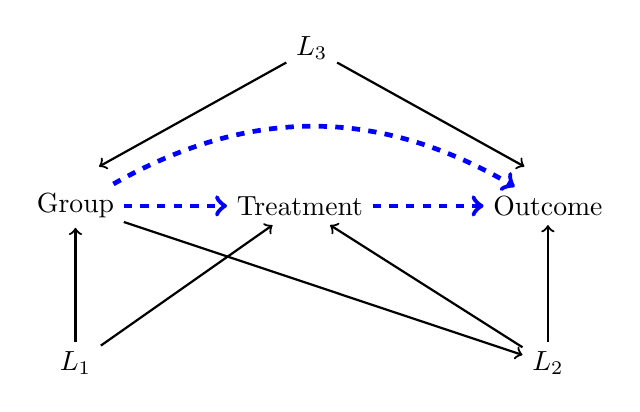
\begin{tikzpicture}[scale = 1] 
    \node at (0,0) {};
    \node at (1,1) {};
    
    \node[anchor = center, align = center] (g) at (0,-1) {Group};
    \node[anchor = center, align=center] (d) at (2.85,-1) {Treatment}; 
    \node[anchor = center, align=center] (y) at (6,-1) {Outcome};   
    \node[anchor = center, align=center] (l1) at (0, -3) {$L_1$};
    \node[anchor = center, align=center] (l2) at (6, -3) {$L_2$};
    \node[anchor = center, align=center] (l3) at (3, 1) {$L_3$};
    
    \draw[->, line width=0.6mm, dashed, blue] (g) to (d);
    \draw[->, line width=0.6mm, dashed, blue] (d) to (y);
    \draw[->, line width=0.6mm, dashed, blue] (g) to [bend left = 30] (y);  
    
    \draw[->, thick] (l1) to (g);  
    \draw[->, thick] (l1) to (d);  
    \draw[->, thick] (l2) to (d);  
    \draw[->, thick] (l2) to (y);  
    \draw[->, thick] (g) to (l2);  
    \draw[->, thick] (l3) to (0.3,-0.5);  
    \draw[->, thick] (l3) to (5.7,-0.5);  
\end{tikzpicture}
}
\subfigure[Group decomposition]
{
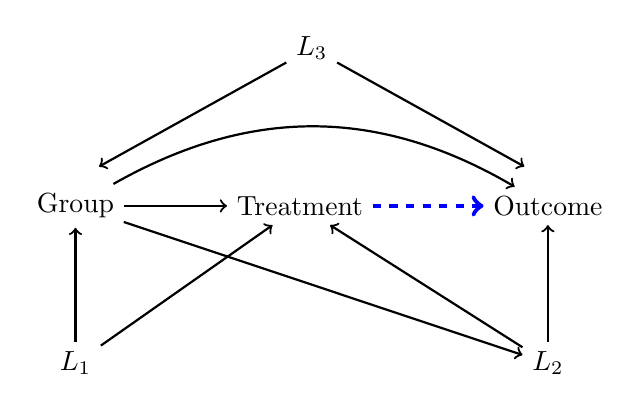
\begin{tikzpicture}[scale = 1]  
    \node at (0,0) {};
    \node at (1,1) {};
    
    \node[anchor = center, align = center] (g) at (0,-1) {Group};
    \node[anchor = center, align=center] (d) at (2.85,-1) {Treatment}; 
    \node[anchor = center, align=center] (y) at (6,-1) {Outcome};   
    \node[anchor = center, align=center] (l1) at (0, -3) {$L_1$};
    \node[anchor = center, align=center] (l2) at (6, -3) {$L_2$};
    \node[anchor = center, align=center] (l3) at (3, 1) {$L_3$};
    
    \draw[->, thick] (g) to (d);
    \draw[->, line width=0.6mm, dashed, blue] (d) to (y);
    \draw[->, thick] (g) to [bend left = 30] (y);  
    
    \draw[->, thick] (l1) to (g);  
    \draw[->, thick] (l1) to (d);  
    \draw[->, thick] (l2) to (d);  
    \draw[->, thick] (l2) to (y);  
    \draw[->, thick] (g) to (l2);  
    \draw[->, thick] (l3) to (0.3,-0.5);  
    \draw[->, thick] (l3) to (5.7,-0.5);  
\end{tikzpicture}
}

\caption*{Figure 1. Causal graphs illustrating the difference in identification between causal mediation analysis and causal decomposition of group disparities. The dashed edges are the paths each framework seeks to identify. Causal mediation analysis aims to identify both the effects of group and treatment, hence requiring proper handling of all three types of confounders: $L_1$, $L_2$, and $L_3$. Our causal decomposition only needs to identify the effect of treatment, so only treatment-outcome confounders, i.e., $L_2$, are of concern.} 

\end{figure}


\subsection{Relation to unconditional random equalization decomposition}
In recent years, there have emerged two variants of random equalization decomposition, each of which further has an unconditional version and a conditional version \citep{vanderweele_causal_2014, jackson_decomposition_2018, sudharsanan_educational_2021, lundberg_gap-closing_2022,park_sensitivity_2023}. In this section, we compare our unconditional decomposition with unconditional random equalization decomposition (URED). URED decomposes the observed disparity into two components. One is the reduction in disparity that could be brought about by randomly reassigning the treatment such that the treatment prevalence is equalized across groups. The other is correspondingly a component of remaining disparity. Similar to our approach, URED is associated with an intervention on treatment, not on group membership. However, URED is a two-way decomposition that contains less information than our four-way decomposition. Moreover, the reduction in disparity in URED combines the selection component and the prevalence component of our decomposition, impeding a clear interpretation.

%%%%% The random equalization decomposition was pioneered by \citet{vanderweele_causal_2014}. \citet{jackson_meaningful_2021} extended it to a conditional version, where the random equalization is only conceived within each level of some conditioning variables $\boldsymbol{Q}$. \citet{lundberg_gap-closing_2022} further proposed a slightly different estimand, where both group $a$ and group $b$ are given $D$ values randomly drawn from the entire sample. For the random equalization decomposition, estimators have been constructed based on regression \citep{vanderweele_causal_2014, jackson_decomposition_2018}, weighting \citep{jackson_meaningful_2021}, Monte Carlo integration \citep{sudharsanan_educational_2021}, as well as the doubly-robust augmented inverse probability weighting \citep{lundberg_gap-closing_2022}, which combines regression with weighting.  %%%%%

The first variant of URED is defined in terms of a random equalization intervention that randomly assigns treatment values of the advantaged group to the disadvantaged group.
Using the randomized intervention notation introduced above, Jackson and VanderWeele 
 (\citeyear{jackson_decomposition_2018}) decompose the observed group disparity into two components:
\begin{gather}
\E_a(Y)-\E_b(Y)=\underbrace{\E_b \left(Y_{R(D \mid G=a)} \right)-\E_b(Y)}_{\text{reduction in disparity}} + \underbrace{\E_a(Y)-\E_b \left(Y_{R(D \mid G=a)} \right)}_{\text{remaining disparity}} .  \nonumber 
\end{gather}
The reduction in disparity is intended to quantify the contribution of differential treatment prevalence across groups. 
However, the random equalization intervention not only equalizes treatment prevalence across groups, but also randomizes the treatment within the disadvantaged group, making any selection into treatment disappear in that group. As a consequence, the reduction in disparity equals the combination of the prevalence component and the group $b$ part of the selection component, i.e., $\E_b(\tau)[\E_a(D)-\E_b(D)]-\Cov_b(D, \tau)$, which follows from Equation (\ref{eqt2}). This leads to an interpretational difficulty, as the reduction in disparity does not purely reflect groupwise variation in treatment prevalence. In particular, if group $a$ is an exact replicate of group $b$, this variant of URED will still contain a non-zero reduction in disparity, as long as $\Cov_b(D, \tau) \neq 0$.

The second variant of URED takes a somewhat different form \citep{lundberg_gap-closing_2022}, whose hypothetical intervention assigns each individual in both groups a treatment value randomly drawn from the pooled population. Hence, this random equalization intervention changes the treatment values in both groups instead of only in the disadvantaged group as in the first variant. The reduction in disparity of this variant  mixes the prevalence component with the selection component, too. To show this, we first note that the outcome disparity can also be decomposed as such: 
\begin{align*}
&\phantom{{}={}} \E_a(Y)-\E_b(Y) \\
&= \E_a(Y_{0})-\E_b(Y_{0}) +  \E(D)[ \E_a(\tau) - \E_b(\tau)]  \\
&\phantom{{}={}} +\E(\tau)[\E_a(D)-\E_b(D)] + \Cov_a(D, \tau) - \Cov_b(D, \tau) \\
&\phantom{{}={}} - [P_a-P_b][\E_a(D) - \E_b(D)][\E_a(\tau)-\E_b(\tau)], 
\end{align*} 
where $\E(\tau)$ and $\E(D)$ are the overall ATE and treatment prevalence, $P_a$ and $P_b$ are the proportions of the population in group $a$ and group $b$.
And the remaining disparity in Lundberg's (\citeyear{lundberg_gap-closing_2022}) unconditional decomposition equals 
$\E_a(Y_{0})-\E_b(Y_{0}) + \E(D)[ \E_a(\tau) - \E_b(\tau)] \nonumber$. It then follows that the reduction in disparity in this variant contains the selection component, $\Cov_a(D, \tau) -  \Cov_b(D, \tau)$. The intuition is that in this random equalization intervention, both group $a$ and group $b$ would get random draws of $D$, thus  selection into treatment is eliminated in both groups, making $\Cov_a(D,\tau)=\Cov_b(D,\tau)=0$.

To conclude, the reduction in disparity in both variants of URED is a mixture of the prevalent component and the selection component of group disparities. This is because URED's underlying interventions both equalize and randomize the treatment. In contrast, as explained in Section 2.2,  the prevalence component in our decomposition is solely concerned with the disparity-reducing impact of an equalization intervention and avoids the influence of a randomization intervention.\footnote{This is also why the RIA of PIE can be translated to the prevalence component, but not to the reduction in disparity component in URED. Both the prevalence component and the RIA of PIE are a difference between two quantities that both contain randomized $D$ values, so both estimands can represent the reduction in disparity resulting from a pure equalization intervention \emph{after} a randomization intervention.} If the goal is to capture the contribution of the unequal treatment prevalence to group disparities, one should prefer using the prevalence component in our decomposition.
 
\subsection{Conditional decomposition}
In this section, we extend our framework to a conditional decomposition whose corresponding interventions are conditional on a vector of variables $\boldsymbol{Q}$. The conditional decomposition is useful as it can shed light on the impact of normatively more desirable or realistically more feasible interventions, when the unconditional intervention appears less so \citep{jackson_meaningful_2021}. For example, it may be meaningful to consider equalizing college admissions conditional on test scores or equalizing medical treatments conditional on comorbidities.
Assuming that the the support of $\Q$ is the same in the two groups and still under Assumption 1,
\begin{align}
    \E_a(Y)-\E_b(Y) &= \underbrace{\E_a(Y_0)-\E_b(Y_0)}_{\text{baseline}} \nonumber \\
    &\phantom{{}={}} + \underbrace{\int [\E_a(D \mid \Q=\q)-\E_b(D \mid \Q=\q)]\E_b(\tau \mid \Q=\q) f_b(\q) \dd \q}_{\text{conditional prevalence}} \nonumber \\
    &\phantom{{}={}} + \underbrace{\int [\E_a(\tau \mid \Q=\q)-\E_b(\tau \mid \Q=\q)] \E_a(D \mid \Q=\q) f_a(\q) \dd \q}_{\text{conditional effect}} \nonumber \\
    &\phantom{{}={}} + \underbrace{\E_a[\Cov_a(D, \tau \mid \Q)] - \E_b[\Cov_b(D, \tau \mid \Q)}_{\text{conditional selection}}] \nonumber \\
    &\phantom{{}={}} + \underbrace{\int \E_a(D \mid \Q=\q) \E_b(\tau \mid \Q=\q) [f_a(\q)-f_b(\q)] \dd \q}_{\text{$\Q$ distribution}}.
\end{align}

The conditional prevalence, effect, and selection components indicate the disparity-reducing impacts of equalizing the corresponding group characteristics within levels of $\Q$. Thus, the conditional decomposition allows researchers to incorporate prior information about the subjects when evaluating potential interventions on treatments or their effects. As policies, the conditional interventions are often more feasible but less influential than the marginal interventions encoded in Equation (\ref{eqt1}). In addition, the ``$\Q$ distribution'' component captures the between-$\Q$ disparity, as opposed to within-$\Q$ disparities reflected in other components, but it should not be interpreted causally.

Similar to the unconditional case, we can also interventionally interpret the conditional decomposition using the randomized intervention notation. 
Let $\E_g(Y_{R(D \mid G=g',\Q)})$ be the mean potential outcome of group $g$ when its members were given treatment values randomly drawn from members of group $g'$ who share the same $\Q$ values with them. We can rewrite this mean potential outcome as follows.
\begin{align}
    \E_g(Y_{R(D \mid G=g',\Q)}) = \E_g(Y_0) + \int \E_g(\tau \mid \Q=\q) \E_{g'}(D \mid \Q=\q) f_g(\q) \dd \q.
\end{align}
It then follows that components of the conditional decomposition can be written in the randomized intervention notation:
\begin{align}
    \E_a(Y)-\E_b(Y)-[\E_a(Y_{R(D \mid G=a,\Q)})-\E_b(Y_{R(D \mid G=b,\Q)})] &= \text{conditional selection} \nonumber \\
    \E_b(Y_{R(D \mid G=a,\Q)}) - \E_b(Y_{R(D \mid G=b,\Q)}) &= \text{conditional prevalence} \nonumber \nonumber \\
    \E_a(Y_{R(D \mid G=a,\Q)}) - \E_b(Y_{R(D \mid G=a,\Q)}) &= \text{conditional effect} + \text{conditional selection} \nonumber \\
    &\phantom{{}={}} + \text{$\Q$ distribution}.
\end{align}

Therefore, a two-step intervention again underlies our conditional decomposition. The first step is a conditional randomization, where the pre-treatment disparity is $\E_a(Y)-\E_b(Y)$ and post-intervention disparity is $\E_a(Y_{R(D \mid G=a,\Q)})-\E_b(Y_{R(D \mid G=b,\Q)})$. Hence, the treatment is randomized within each $\Q$ level for members of both groups, and the resulting reduction in disparity is the conditional selection component. 
For the second step, the pre-intervention disparity is $\E_a(Y_{R(D \mid G=a,\Q)})-\E_b(Y_{R(D \mid G=b,\Q)})$ and the post-intervention disparity is $\E_a(Y_{R(D \mid G=a,\Q)}) - \E_b(Y_{R(D \mid G=a,\Q)})$.
The second step is thus a conditional equalization within $\Q$ levels given the prior conditional randomization, and the reduction in disparity is the conditional prevalence component.
What would remain after this two-step intervention is the sum of the conditional effect, the conditional selection, and the $\Q$ distribution components.\footnote{For equation (4) to hold, we only require $\text{supp}_g(\Q) 	\subseteq \text{supp}_{g'}(\Q)$, not necessarily $\text{supp}_g(\Q) = \text{supp}_{g'}(\Q)$ required for the decomposition (3) itself. This implies that the interventional interpretations for conditional selection and conditional prevalence in equation (5) hold as long as $\text{supp}_b(\Q) \subseteq \text{supp}_{a}(\Q)$. Intuitively, at each level of $\Q$ in group $b$, we must be able to find members of group $a$ with the same $\Q$ values in order to conduct the equalization intervention.}

\citet{jackson_meaningful_2021} and \citet{lundberg_gap-closing_2022} proposed two variants of conditional random equalization decomposition (CRED), which again decomposes outcome disparities into a reduction in disparity component and a remaining disparity component. The hypothetical intervention underlying CRED is a random reassignment of treatment values for people with the same $\Q$ values such that treatment prevalence would be equalized within $\Q$ levels. Analogous to the unconditional case, we show that the reduction in disparity component in both variants of CRED does not purely capture differential prevalence of treatment conditional on $\Q$. Therefore, the conditional prevalence component in our decomposition should be preferred for its clearer interpretation. 

In Jackson's (\citeyear{jackson_meaningful_2021}) variant of CRED, the reduction in disparity is $\E_b(Y_{R(D \mid G=a, \Q)})-\E_b(Y)$, which we can rewrite as 
\begin{gather}
\int  [\E_a(D \mid \Q=\q) - \E_b(D \mid \Q=\q)] \E_b(\tau \mid \Q=\q) f_b(\q) \dd \q - \E_b[\Cov_b(D, \tau \mid \Q)]. 
\end{gather}
Therefore, the reduction in disparity is the sum of the conditional prevalence component and the group $b$ part of the conditional selection component. Namely, it captures not only differential treatment prevalence within $\Q$ levels but also the extent of conditional selection into treatment in group $b$. Intuitively, this is because the intervention of this CRED involves both a conditional equalization and a conditional randomization, and the randomization part eliminates selection into treatment conditional on $\Q$ in group $b$. 

A similar case can be shown for the reduction in disparity in the CRED of \citet{lundberg_gap-closing_2022}.
\begin{align}
&\phantom{{}={}} \E_a(Y)-\E_b(Y) \nonumber \\ 
&\phantom{{}={}} \left\lbrace \E_a[\Pro(D=0 \mid \Q) Y_0 + \Pro(D=1 \mid \Q) Y_1] - \E_b[\Pro(D=0 \mid \Q) Y_0 + \Pro(D=1 \mid \Q) Y_1] \right\rbrace \nonumber \\
&= \E_a[\Cov_a(D,\tau \mid \Q)] - \E_b[\Cov_b(D,\tau \mid \Q)] + \int [\E_a(D \mid \Q=\q) - \E_b(D \mid \Q=\q)] \nonumber \\
&\phantom{{}={}} [\E_a(\tau \mid \Q=\q)f_a(\q)\Pro(G=b \mid \Q=\q) + \E_b(\tau \mid \Q=\q)f_b(\q)\Pro(G=a \mid \Q=\q)] \dd \q,
\end{align}
where the left hand side is the reduction in disparity in Lundberg's CRED. Hence, the reduction in disparity involves both a term for differential treatment prevalence within $\Q$ levels and the conditional selection component. The intervention in this case corresponds to the combination of a conditional equalization and a conditional randomization in both groups. Consequently, both differential treatment prevalence and differential selection into treatment would be reduced to zero conditional on $\Q$. Distinct from the reduction in disparity in both variants of CRED, the conditional prevalence component in our decomposition solely measures the impact of a conditional equalization intervention. By implication, only our conditional prevalence component can be interpreted as a pure measure of the contribution of differential treatment prevalence within $\Q$ levels to  outcome disparities. 


\section{Estimation and Inference}
We identify the components of our decompositions using two standard assumptions as follows.
\begin{itemize}
    \item[] Assumption 2 (Conditional ignorability). $Y_d \indep D \mid \X=\x, G=g$, $\forall d, \x, g$;
    \item[] Assumption 3 (Overlap). $0 < \E(D \mid \X=\x, G=g) <1$, $\forall \x, g$.
\end{itemize}
Without loss of generality, we assume $\Q \in \X$. 
We develop nonparametric and efficient estimators for our unconditional and conditional decompositions.\footnote{Various regression, weighting, or matching estimators can also be used. Also note that, under constant treatment effect, the prevalence component in the unconditional decomposition can be estimated using the traditional ``product method'' for the indirect effect of $G$ through $D$ on $Y$ \citep{baron_moderator-mediator_1986}. This again explicates the kinship between our decomposition and mediation analysis. }
These estimators are ``one-step'' estimators based on the EIFs of the decomposition components, which remove the bias from naive substitution estimators \citep{bickel_efficient_1998, van_der_vaart_asymptotic_2000,hines_demystifying_2022}. The estimators contain some nuisance functions, which can be estimated using flexible ML methods coupled with cross-fitting. Under specified conditions, our estimators are $\sqrt{n}$-consistent, asymptotically normal, and semiparametrically efficient. Thus, we are able to construct asymptotically accurate Wald-type confidence intervals and hypothesis tests. Our estimators also have double robustness properties.  

To introduce the EIFs, we define the following functions:
\begin{align*}
    \mu(d,\X, g)&=\E(Y \mid D, \X, G=g) \\
    \pi(d,\X, g) &= \Pro(D=d \mid \X, G=g) \\
    p_g &= \Pro(G=g) \\
    p_g(\Q) &= \Pro(G=g \mid \Q).
\end{align*}
Below, we use $\xi$ to denote the estimands (decomposition components), $\phi$ to denote the EIFs, and $\Psi$ to denote the resulting one-step estimators. 

\subsection{The unconditional decomposition}
All components of the unconditional decomposition are simple linear combinations of the total disparity and two generic functions evaluated at appropriate values of $d$, $g$, and $g'$: $\xi_{dg} \defeq \E \left(Y_d \mid G=g  \right)$ and $\xi_{dgg'} \defeq \E \left(Y_d \mid G=g \right)\E \left(D \mid G=g' \right)$. The relationship between components of the unconditional decomposition and the generic functions is as follows:
\begin{align*}
    \text{Baseline} &= \xi_{0a}-\xi_{0b}  \\
    \text{Prevalence} &= \xi_{1ba}-\xi_{0ba}-\xi_{1bb}+\xi_{0bb} \\
    \text{Effect} &= \xi_{1aa}-\xi_{0aa} - \xi_{1ba}+\xi_{0ba} \\
    \text{Selection} &= \text{Total} - \text{Baseline} - \text{Prevalence} - \text{Effect} .
\end{align*}
Hence, the EIFs and one-step estimators for the decomposition components directly follow from those of $\xi_{dg}$ and $\xi_{dgg'}$. In addition, these generic functions also provide a basis for estimating Jackson's (\citeyear{jackson_decomposition_2018}) version of the unconditional equalization estimand, since its reduction in disparity component can be represented as $\xi_{0b} + \xi_{1ba}-\xi_{0ba}-\E_b(Y)$. Under Assumptions 1, 2, and 3, $\xi_{dg}$ and $\xi_{dgg'}$ can be identified as the following quantities:
\begin{align*}
    \xi_{dg} &= \E \left[\mu(d,\X,g) \mid G=g \right] \\
    \xi_{dgg'} &= \E \left[\mu(d,\X,g) \mid G=g \right] \E \left[D \mid G=g' \right].
\end{align*}

These identification results then enable us to derive the EIFs for $\xi_{dg}$ and $\xi_{dgg'}$.
\begin{prop}[EIF, unconditional decomposition]
Under Assumptions 1, 2, and 3, the EIF of $\xi_{dg}$ is
$$\phi_{dg}(Y,\X) \defeq \frac{\one(G=g)}{p_g} \left\{ \frac{\one(D=d)}{\pi(d, \X,g)} [Y-\mu(d,\X,g)] + \mu(d,\X,g) - \xi_{dg} \right\},$$ 
and the EIF of $\xi_{dgg'}$ is
\begin{align*}
    \phi_{dgg'}(Y,\X) &\defeq \frac{\one(G=g)}{p_g}  \left\{\frac{\one(D=d)}{\pi(d,\X,g)}[Y-\mu(d,\X,g)] + \mu(d,\X,g) \right\} \E \left(D \mid G=g' \right) \\
    &\phantom{{}={}} + \frac{\one(G=g')}{p_{g'}} \E \left(Y_d \mid G=g \right) \left[D - \E \left(D \mid G=g' \right) \right] - \frac{\one(G=g)}{p_g} \xi_{dgg'}.
\end{align*}
In Appendix B, we derive the EIFs for the general case with survey weights for both unconditional and conditional decompositions. 
\end{prop}
It follows that the one-step estimators are
\begin{align*}
    \Psi_{dg}(Y,\X) &\defeq \frac{1}{n} \sum \frac{\one(G=g)}{p_g} \left\{ \frac{\one(D=d)}{\pi(d, \X,g)} [Y-\mu(d,\X,g)] + \mu(d,\X,g)\right\} \\
    \Psi_{dgg'}(Y,\X) &\defeq \frac{1}{n} \sum \frac{\one(G=g)}{p_g}  \left\{\frac{\one(D=d)}{\pi(d,\X,g)}[Y-\mu(d,\X,g)] + \mu(d,\X,g) \right\} \E \left(D \mid G=g' \right).
\end{align*}
There are two nuisance functions, $\pi(d,\X,g)$ and $\mu(d,\X,g)$. In order to relax the conditions required of nuisance function models, we use cross-fitting to estimate all nuisance functions \citep{kennedy_semiparametric_2022, chernozhukov_double/debiased_2018}. In particular, we first divide the sample randomly into two subsamples. Then we fit the nuisance functions using each subsample. Finally, we evaluate the fitted nuisance functions using data not in the subsample used to fit the functions. In practice, to improve the finite-sample performance of the estimator, we may stabilize the weights by dividing $\one(D=d)/\pi(d,\X,g)$ by its sample average.  

To study the asymptotic behavior of the one-step estimators for the unconditional decomposition, we invoke three additional assumptions,\footnote{Throughout this paper, the consistent estimation of $p_g$ and $\E(D \mid G=g), \forall g,$ is left implicit.} which are consistent with assumptions required for the double ML estimator of ATE \citep{kennedy_semiparametric_2022, chernozhukov_double/debiased_2018}. We let $\| \cdot \|$ denote the $L_2$-norm. 

Assumption 4a (Boundedness). With probability 1, $\hat{\pi}(d,\X,g) \geq \eta$, $\pi(d,\X,g) \geq \eta$, and $|Y-\hat{\mu}(d,\X,g)| \leq \zeta$, for some $\eta>0$ and some $\zeta < \infty$, $\forall d, g$.

Assumption 5a (Consistency).  $\| \hat{\mu}(d,\X,g) - \mu(d,\X,g) \| =o_p(1)$ and $\| \hat{\pi}(d,\X,g) - \pi(d,\X,g) \| =o_p(1)$, $\forall d, g$.

Assumption 6a (Convergence rate).  $\|\hat{\pi}(d,\X,g)-\pi(d,\X,g)\| \|\hat{\mu}(d,\X,g)-\mu(d,\X,g)\|=o_p(n^{-1/2})$, $\forall d, g$.

\begin{prop}[Asymptotic distribution, unconditional decomposition]
Under Assumptions 1, 2, 3, 4a, 5a, and 6a, the one-step estimators for components of the unconditional decomposition are asymptotically normal and semiparametrically efficient, i.e., $\sqrt{n}(\Psi_{dg} - \xi_{dg}) \xrightarrow{d} \mathcal{N}(0, \sigma^2_{dg})$, and $\sqrt{n}(\Psi_{dgg'} - \xi_{dgg'}) \xrightarrow{d} \mathcal{N}(0, \sigma^2_{dgg'})$, where $\sigma^2_{dg}=\E[\phi_{dg}(Y,\X)^2]$ and $\sigma^2_{dgg'}=\E[\phi_{dgg'}(Y,\X)^2]$ are the respective semiparametric efficiency bounds. 
\end{prop}
Assumptions 4a through 6a are mild in the sense that they are often satisfied by popular ML models. The desirable asymptotic properties also carry over from $\Psi_{dg}$ and $\Psi_{dgg'}$ to the final estimators of the decomposition components. We consistently estimate $\sigma^2_{dg}$ and $\sigma^2_{dgg'}$ using the  averages of squared estimated EIFs. The asymptotic distributions can then be used to construct hypothesis testing and confidence intervals. For example, a Wald-style $1-\alpha$ confidence interval for the prevalence component is $$\Psi_{1ba}-\Psi_{1bb}-\Psi_{0ba}+\Psi_{0bb} \pm z_{1-\alpha/2} \cdot \frac{1}{n} \left[\sum  \left(\hat{\phi}_{1ba}-\hat{\phi}_{1bb}-  \hat{\phi}_{0ba}+\hat{\phi}_{0bb}\right)^2 \right]^{1/2}.$$ Furthermore, our estimators also have a double robustness property. 

\begin{prop}[Double robustness, unconditional decomposition]
Either consistent estimation of $\mu(d,\X,g)$ or $\pi(d,\X,g)$ for all $d$ and $g$ is sufficient for the consistency of $\Psi_{dg}$ and $\Psi_{dgg'}$.  
\end{prop}
Hence, our unconditional decomposition estimator only requires the same conditions as the classic augmented inverse probability weighting estimator for ATE \citep{robins_estimation_1994, hirano_efficient_2003} to be consistent. 

\subsection{The conditional decomposition}
Relative to the unconditional case, we only need to additionally consider one generic function:
$$\xi_{dgg'g''} \defeq \E \left[\E \left(Y_d   \mid \Q, g \right) \E \left(D \mid \Q, g' \right) \mid G=g'' \right],$$
where $(d, g, g', g'')$ is any combination of treatment status and group memberships out of 8 possible combinations. The relationship between components of the conditional decomposition and the generic functions is as follows:
\begin{align*}
    \text{Baseline} &= \xi_{0a}-\xi_{0b}  \\
    \text{Conditional Prevalence} &= \xi_{1bab}-\xi_{0bab}-\xi_{1bbb}+\xi_{0bbb} \\
    \text{Conditional Effect} &= \xi_{1aaa}-\xi_{0aaa} - \xi_{1baa}+\xi_{0baa} \\
    \Q \text{ Distribution} &= \xi_{1baa}-\xi_{0baa} - \xi_{1bab}+\xi_{0bab} \\
    \text{Conditional Selection} &= \text{Total} - \text{Baseline} \\
    &\phantom{{}={}} - \text{Conditional Prevalence} - \text{Conditional Effect} - \Q \text{ Distribution}.
\end{align*}
Hence, we now focus on the inference of $\xi_{dgg'g''}$. The EIFs,  one-step estimators, and their asymptotic distributions for components of the conditional decomposition will then follow. Moreover, we thereby also provide nonparametric inference for the reduction in disparity component in the CRED of \citet{jackson_meaningful_2021}, which can be represented as $\xi_{0b}+\xi_{1bab}-\xi_{0bab}-\E_b(Y)$.
Under assumptions 1, 2, 3, we identify $\xi_{dgg'g''}$ as $$\E \left\{\E \left[ \E(Y \mid d,\X,g)   \mid \Q, g \right] \E \left(D \mid \Q, g' \right) \mid G=g'' \right\}.$$

\begin{prop}[EIF, conditional decomposition]
Under Assumptions 1, 2, 3, the EIF of $\xi_{dgg'g''}$ is 
\begin{align*}
     &\phantom{{}={}} \phi_{dgg'g''}(Y,\X,\Q) \\
    &=\frac{\one(G=g'')}{p_{g''}} \left[ \E \left(Y_d \mid \Q, g \right) \E \left(D \mid \Q, g' \right) - \xi_{dgg'g''} \right] \\
    &\phantom{{}={}} + \frac{\one(G=g) p_{g''}(\Q)}{p_g(\Q)p_{g''}} \left\{ \frac{\one(D=d)}{\pi(d,\X,g)} [Y-\mu(d,\X,g)]+\mu(d,\X,g) - \E \left(Y_d \mid \Q,g \right) \right\} \E \left(D \mid \Q,g' \right) \\
    &\phantom{{}={}} + \frac{\one(G=g')p_{g''}(\Q)}{p_{g'}(\Q)p_{g''}} \left[ D-\E \left(D \mid \Q, g' \right) \right] \E\left( Y_d \mid \Q, g \right).
\end{align*}
\end{prop}
We again construct the one-step estimator based on the EIF. 
\begin{align*}
    &\phantom{{}={}} \Psi_{dgg'g''}(Y,\X,\Q) \\
    &=\frac{\one(G=g'')}{p_{g''}} \E \left(Y_d \mid \Q, g \right) \E \left(D \mid \Q, g' \right) + \frac{\one(G=g')p_{g''}(\Q)}{p_{g'}(\Q)p_{g''}} \left[ D-\E \left(D \mid \Q, g' \right) \right] \E\left( Y_d \mid \Q, g \right) \\
    &\phantom{{}={}} + \frac{\one(G=g) p_{g''}(\Q)}{p_g(\Q)p_{g''}} \left\{ \frac{\one(D=d)}{\pi(d,\X,g)} [Y-\mu(d,\X,g)]+\mu(d,\X,g) - \E \left(Y_d \mid \Q,g \right) \right\} \E \left(D \mid \Q,g' \right).
\end{align*}
For this estimator, there are five nuisance functions: $p_g(\Q)$, $\pi(d,\X,g)$, $\mu(d,\X,g)$, $\E(D \mid \Q, g)$, and $\E(Y_d \mid \Q,g)$. We again cross-fit these nuisance functions using nonparametric methods. This estimator can be weight-stabilized by dividing $\one(D=d)/\pi(d,\X,g)$, $\one(G=g')p_{g''}(\Q)/p_{g'}(\Q)p_{g''}$, and $\one(G=g)p_{g''}(\Q)/p_g(\Q)p_{g''}$ by their respective sample averages. The estimation of $\E(Y_d \mid \Q,g)=\E[\mu(d,\X,g) \mid \Q,g]$ requires a more involved procedure. We adopt a pseudo-outcome approach \citep[e.g.,][]{van_der_laan_statistical_2006,semenova_debiased_2021}, where the pseudo outcome for each $d$ is defined as the decentered EIF for $\E(Y_d)$, i.e., 
$$ \delta_d \left(Y, \X,  G \right) \defeq \frac{\one(D=d)}{\pi(d, \X,G)} [Y-\mu(d,\X,G)] + \mu(d,\X,G).$$
We first estimate $\pi(d, \X,G)$ and $\mu(d,\X,G)$ within two random subsamples of the data \emph{without} cross-fitting and obtain the estimated pseudo outcome $\hat{\delta}_d \left(Y, \X,  G \right)$. Then, using $\hat{\delta}_d \left(Y, \X,  G \right)$ as a proxy of $Y_d$, we estimate $\E\left[Y_d \mid \Q, g \right]$ \emph{with} cross-fitting, i.e., we fit $\E\left[\hat{\delta}_d \left(Y, \X,  G \right) \mid \Q, g \right]$ in one subsample and plug in values of $\Q$ in the other subsample. Using this procedure, we ensure that the fitting of $\E(Y_d \mid \Q,g)$, which relies on estimating the pseudo outcome, is done separately in each subsample. 

The asymptotic theory of the one-step estimator for $\xi_{dgg'g''}$ is less general than the theories for $\xi_{dg}$ and $\xi_{dgg'}$, in that some conditions differ by the specific configuration of $g, g'$ and $g''$. Note that  $g=g''$ for the conditional prevalence component, and $g'=g''$ for the conditional effect component. For $\sqrt{n}$-consistency, asymptotic normality, and efficiency, we need three assumptions. 

Assumption 4b (Boundedness). With probability 1,  $\hat{\pi}(d,\X,g) \geq \eta$, $\pi(d,\X,g) \geq \eta$, $\hat{p}_g(\Q) \geq \eta$, $p_g(\Q) \geq \eta$, 
$|Y-\hat{\mu}(d,\X,g)| \leq \zeta$, 
$|Y-\mu(d,\X,g)| \leq \zeta$, 
$|\mu(d,\X,g)| \leq \zeta$,
$|\E(Y_d \mid \Q,g)| \leq \zeta$, and $\left| \frac{\hat{p}_g(\Q)}{\hat{p}_{g'}(\Q)} \right| \leq \zeta$, for some $\eta>0$ and $\zeta < \infty$, $\forall d,g,g'$.

Assumption 5b (Consistency). $\| \hat{\mu}(d,\X,g) - \mu(d,\X,g) \| =o_p(1)$, $\| \hat{\pi}(d,\X,g) - \pi(d,\X,g) \| =o_p(1)$, $\left\| \hat{\E}(Y_d \mid \Q,g) - \E(Y_d \mid \Q,g) \right\| =o_p(1)$, $\left\| \hat{\E}(D \mid \Q,g) - \E(D \mid \Q,g) \right\| =o_p(1)$, and $\left\| \hat{p}_g(\Q) -p_g(\Q) \right\|=o_p(1)$, $\forall d,g$.

Assumption 6b (Convergence rate). $\left\|\hat{\pi}(d,\X,g)-\pi(d,\X,g) \right\| \|\hat{\mu}(d,\X,g)-\mu(d,\X,g)\|=o_p(n^{-1/2})$, $\left\| \one(G=g) \E(Y_d \mid \Q,g) - \one(G=g')\frac{\hat{p}_{g}(\Q)}{\hat{p}_{g'}(\Q)} \hat{\E}( Y_d \mid \Q, g ) \right\| \left\| \hat{\E}(D \mid \Q, g') - \E(D \mid \Q, g') \right\| = o_p(n^{-1/2})$, and $\left\| \one(G=g') \E(D \mid \Q,g') - \one(G=g) \frac{\hat{p}_{g'}(\Q) }{\hat{p}_g(\Q) } \hat{\E}(D \mid \Q,g') \right\| \left\| \hat{\E}(Y_d \mid \Q,g) - \E(Y_d \mid \Q,g)  \right\| = o_p(n^{-1/2})$, $\forall d,g,g'$.

\begin{prop}[Asymptotic distribution, conditional decomposition]
Under Assumptions 1, 2, 3, 4b, 5b, 6b, the one-step estimator for components of the conditional decomposition is asymptotically normal and semiparametrically efficient, i.e., $\sqrt{n} \left( \Psi_{dgg'g''} - \xi_{dgg'g''} \right) \xrightarrow{} \mathcal{N}(0, \sigma^2_{dgg'g''})$, where $\sigma^2_{dgg'g''}=\E \left[\phi_{dgg'g''}(Y,\X,\Q)^2 \right]$ is the semiparametric efficiency bound.
\end{prop}
Some further insights can be gained about the second and third convergence rate assumptions. For a specific $\xi_{dgg'g''}$, first, when $g=g'=g''$, $\left\| \hat{\E}\left( Y_d \mid \Q, g \right) - \E(Y_d \mid \Q,g)  \right\| \left\| \hat{\E}(D \mid \Q, g) - \E(D \mid \Q, g)  \right\| = o_p(n^{-1/2})$ is sufficient. Hence, we obtain a form of rate double robustness with respect to $\E(Y_d \mid \Q,g)$ and $\E(D \mid \Q, g)$. Second, when $g= g'' \neq g'$, the following set of conditions is sufficient: for a constant $\zeta>0$, $\hat{p}_g(\Q)/\hat{p}_{g'}(\Q) \leq \zeta$ with probability 1, $\left\| \hat{\E}(D \mid \Q, g') - \E(D \mid \Q, g') \right\|=o_p(n^{-1/2})$, and $ \left\| \hat{\E}\left( Y_d \mid \Q, g \right) - \E(Y_d \mid \Q,g) \right\|=o_p(1)$. Third, when $g'=g'' \neq g$, a sufficient set is: for a constant $\zeta>0$, $ \hat{p}_{g'}(\Q)/\hat{p}_{g}(\Q) \leq \zeta$ with probability 1, $\left\| \hat{\E}(D \mid \Q, g') - \E(D \mid \Q, g') \right\|=o_p(1)$, and $\left\| \hat{\E}\left( Y_d \mid \Q, g \right) - \E(Y_d \mid \Q,g)  \right\|=o_p(n^{-1/2})$. Therefore, the assumption is weaker for the inference of the conditional prevalence component, which is also the case for Theorem 6 below.

\begin{prop}[Double robustness, conditional decomposition]
We assume consistent estimation of $\E(D \mid \Q, g), \forall g$. For a $\xi_{dgg'g''}$, when $g=g''$, consistent estimation of either $\mu(d,\X,g)$ or $\pi(d,\X,g)$ is sufficient for the consistency of $\Psi_{dgg'g''}$; when $g \neq g''$, if the estimation of $\E(Y_d \mid \Q,g)$ is doubly robust with respect to $\mu(d,\X,g)$ and $\pi(d,\X,g)$, then consistent estimation of either $\mu(d,\X,g)$ or $\pi(d,\X,g)$ is still sufficient for the consistency of $\Psi_{dgg'g''}$.
\end{prop}
Note that consistent estimation of $\hat{p}_g(\Q)$ is not required for the consistency of $\Psi_{dgg'g''}$. The double robustness condition for $\E(Y_d \mid \Q,g)$ in the case of $g \neq g''$ motivates our pseudo-outcome estimator of $\E(Y_d \mid \Q,g)$, which is built on both $\mu(d,\X,g)$ and $\pi(d,\X,g)$.

For both the unconditional and conditional decompositions, the cdgd package offers various options for nuisance function estimation, including various ML methods, a parametric option using linear and logistic regressions, and an option that allows users to manually plug in nuisance function estimates.


\section{Application}
\subsection{Overview}
We apply our causal decomposition to investigate the role of college graduation in intergenerational income mobility in the United States. In this empirical setting, groups are defined by parental income, the outcome  is adult income, and the treatment is college graduation. 
Previous research has touched upon the components of our unconditional decomposition to various degrees, but this is the first study to comprehensively evaluate the three distinct ways in which college graduation might contribute to the intergenerational transmission of income advantages. 

The baseline component represents the part of the income attainment disparity that is unaccounted for by college graduation. Apart from college completion, parental income is associated with a variety of pre-college characteristics that have direct bearings on income attainment, such as cognitive skills and noncognitive traits in adolescence \citep{reardon_widening_2011, heckman_effects_2006, farkas_cognitive_2003}. Moreover, in adulthood, people from more privileged backgrounds may continue to benefit from various resources passed on within their families regardless of formal educational attainment. Any intervention imposed on the post-secondary credentialing process cannot eliminate channels of income persistence that are independent of college graduation. 

Conceptually in line with the prevalence component in our decomposition, social scientists have long construed education as a mediator of the intergenerational reproduction of SES inequalities (\citealp[chapter 4 \& 5]{blau_american_1978}; \citealp[p.255-9]{featherman_opportunity_1978}; \citealp{ishida_class_1995}; \citealp{breen_educational_2010}). In particular, researchers have documented large and widening income gaps in college graduation \citep{ziol-guest_parent_2016, bailey_gains_2011}. Using a descriptive simulation, \citet{bloome_educational_2018} concluded that rising educational inequality strengthened intergenerational income persistence over time. 

There is also an active literature on the heterogeneity of the college effect on SES attainment by SES origin, which underpins our effect component. Brand et al. (\citeyear{brand_uncovering_2021}) and Cheng et al. (\citeyear{cheng_heterogeneous_2021}) found that the college premiums on wage and income outcomes are larger for people who are economically disadvantaged in adolescence. However, Zhou (\citeyear{zhou_equalization_2019}) and Fiel (\citeyear{fiel_great_2020}) found only insignificant heterogeneity in the effect of college completion on income by parental income. However, these works did not evaluate the extent to which income disparities can be attributed to groupwise differential effects of college.

Finally, findings have been mixed on the direction of selection into college completion based on college effects on SES attainments, i.e., the sign of $Cov(D, \tau)$. Brand and Xie (\citeyear{brand_who_2010}) and Brand et al. (\citeyear{brand_uncovering_2021}) concluded that there is negative selection into college. However, Breen et al. (\citeyear{breen_heterogeneous_2015}) cautioned that Brand and Xie's (\citeyear{brand_who_2010}) result may be biased from unobserved confounding. The instrumental variable analysis of Heckman et al. (\citeyear{heckman_returns_2018}), on the other hand, reveals positive selection. This line of inquiry does not estimate group-specific selection patterns, thereby missing the linkage between group-differentiated selection and outcome disparities. In Appendix E, we clarify and synthesize the differences and connections between various concepts of ``selection into college'' in the social science literature. 

\subsection{Data, variables and estimation details}
We analyze the National Longitudinal Survey of Youth 1979 (NLSY79), which is a nationally representative dataset for a cohort of people who were born between 1957 and 1964 and were living in the United States at the baseline survey in 1979.
We restrict the sample to respondents who were between 14 to 17 years old in 1979 to ensure that income origin is measured before the respondents had a chance to graduate from college. We also limit the analysis to high school graduates by age 29. After deleting individuals with missing values, the final sample size is 2,008. Missingness mostly occurs in the outcome variable due to loss to follow up, where 22\% are missing, while other variables have fewer than 6\% missing values.

We contrast income-origin groups defined as the top 40\% and bottom 40\% of family incomes averaged over the first three waves of the survey (1979, 1980, and 1981) and divided by the square root of the family size. The respondents were 14 to 20 years old during that time. The treatment variable is a binary indicator of whether the respondent graduated from college by age 29. We measure the outcome by percentile rank of adult incomes, averaged over five survey waves between age 35 and 44 and again divided by the square root of family size. For the conditional decomposition, we define $\Q$ to be the Armed Forces Qualification Test (AFQT) score measured in 1980, which reflects academic achievement in high school. 

Baseline covariates used for causal identification ($\X$ variables) include gender, race, parental income percentile, parental education, parental presence, the number of siblings, urban residence, educational expectation, friends' educational expectation, AFQT score, age at baseline survey, the Rotter score of control locus, the Rosenberg self-esteem score, language spoken at home, urban/rural residence, presence of mother, school satisfaction, region of residence, and mother's working status. 

We fit the nuisance functions using three alternative ML methods, gradient boosting machine (GBM), neural networks and random forests. For comparison, we also fit the nuisance functions using parametric regressions. The parametric models are set up as follows. For models predicting $Y$, we use linear regressions with all two-way interactions between the treatment and  baseline variables including the group indicator, along with their main effects. For propensity score models and models predicting $G$, the covariates are entered linearly. For other models, where only $G$ and $\Q$ are predictors, we include all main effects and two-way interactions between $G$ and $\Q$.\footnote{Code for this analysis is available at \url{https://github.com/ang-yu/causal_decomposition_case_study}.}

\subsection{Results}

\begin{figure}
\centering

\subfigure[Unconditional decomposition]
{
\begin{tikzpicture}[scale = 1] 
    \node at (0,0) {};
    \node at (1,1) {};
    
    \node[anchor=center, align=center, inner sep=0pt] at (0,0) {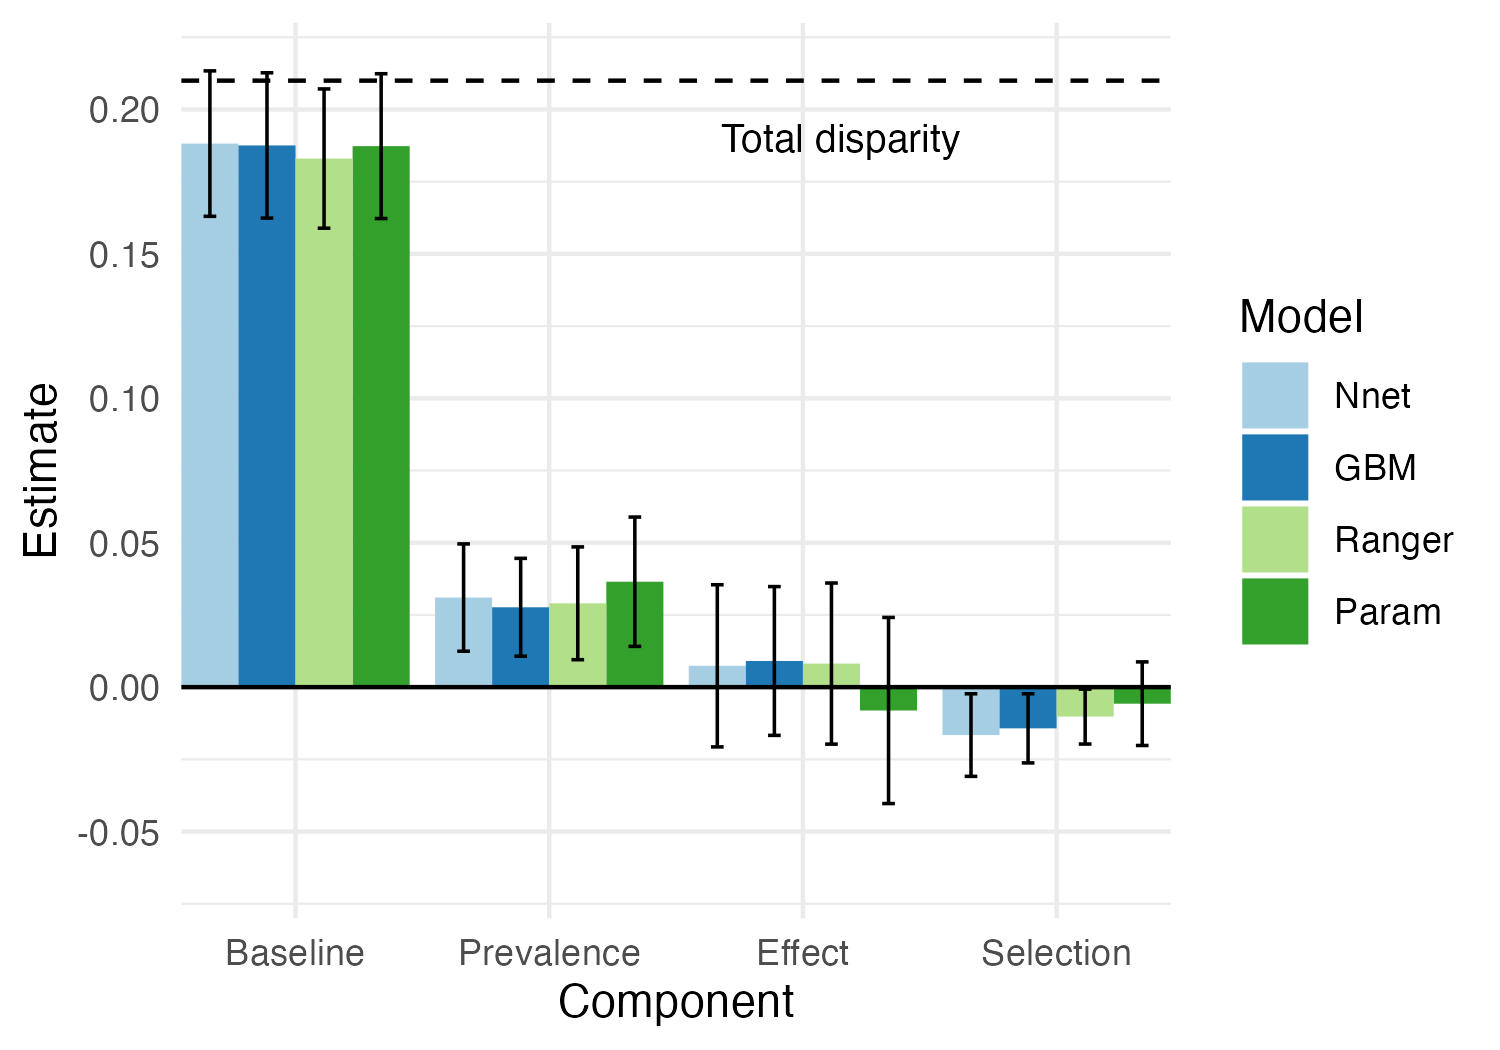
\includegraphics[width=.48\textwidth]{unconditional_2023-06-04.jpg}};
\end{tikzpicture}
}
\subfigure[Conditional decomposition]
{
\begin{tikzpicture}[scale = 1]  
    \node at (0,0) {};
    \node at (1,1) {};
    
    \node[anchor=center, align=center, inner sep=0pt] at (0,0) {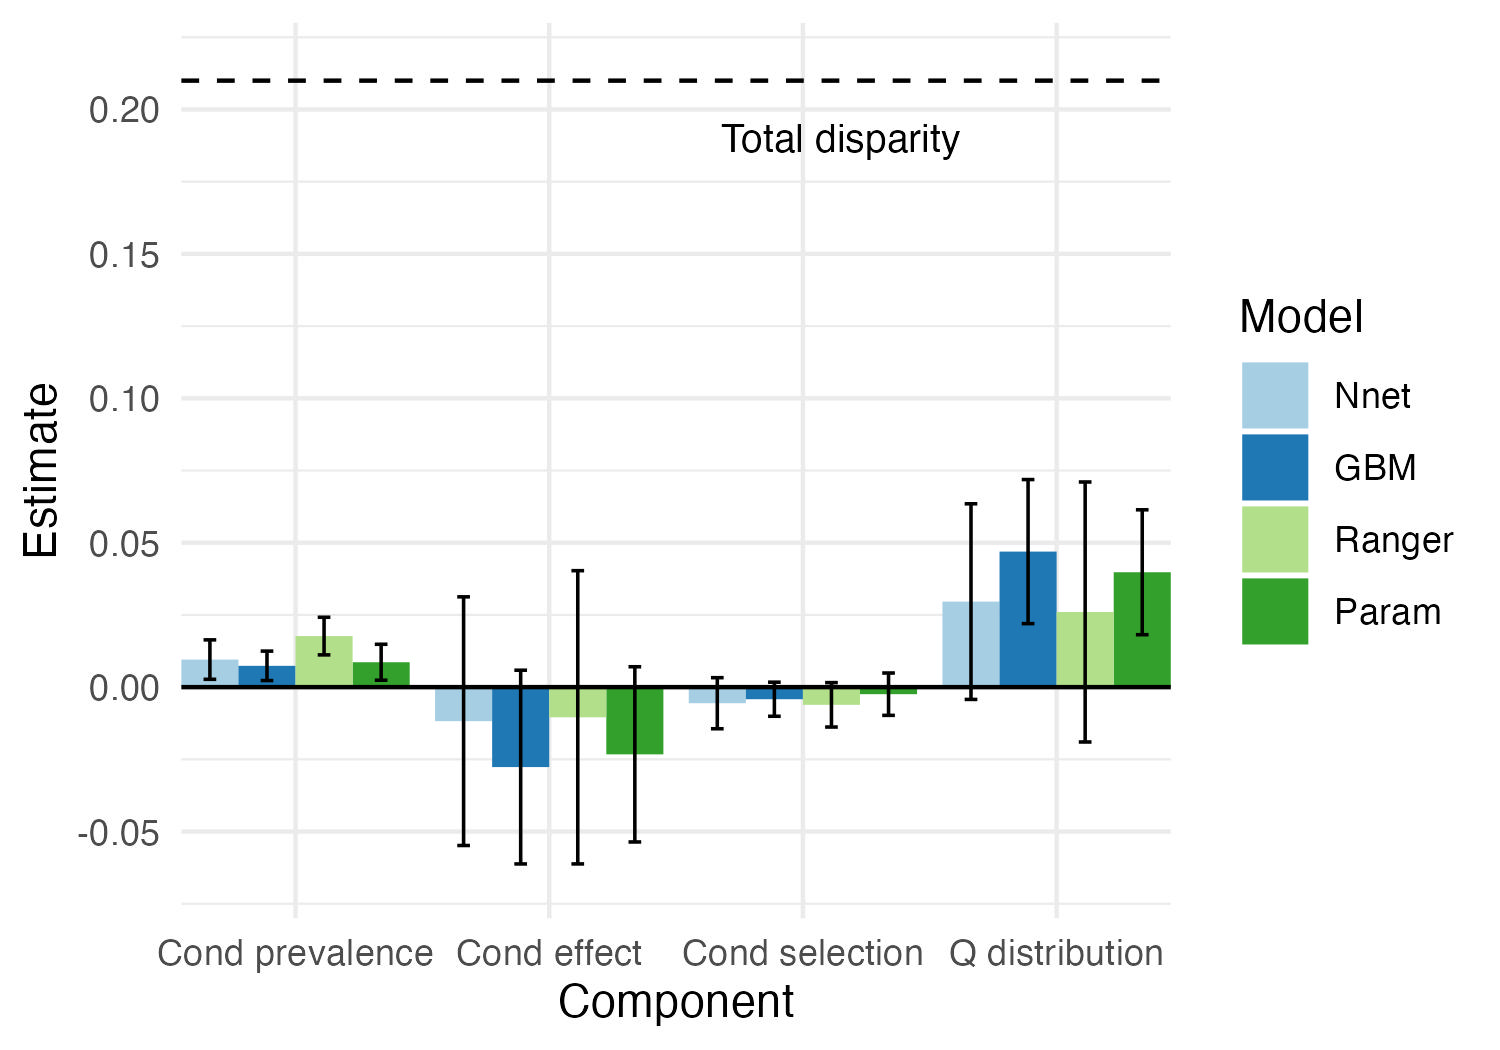
\includegraphics[width=.48\textwidth]{conditional_2023-06-04.jpg}}; 
\end{tikzpicture}
}

\caption*{Figure 2. Decomposition estimates. Cond=conditional, Para=parametric models, Nnet=neural networks, GBM=generalized boosting machine, Ranger=random forests. Error bars indicate 95\% confidence intervals. Baseline component is omitted in panel (b) as the baseline component estimates for the conditional decomposition are, by definition, the same as those for the unconditional decomposition.} \label{fig:Result}
\end{figure}

We illustrate estimates of the decompositions in Figure 2, while the numeric estimates are presented in Appendix Table A2 and A3. To aid the interpretation of the decomposition components, in Appendix Table A1, we additionally report estimated group-specific means of baseline potential outcome, treatment proportion, ATE, and covariance between treatment and treatment effect, as well as group differences in these quantities. 

To begin with, according to the estimated total disparity, people from lower income origin on average achieve 21 percentiles lower incomes in their 30s and 40s. This confirms the well-established pattern of integenerational income persistence. Our decompositions reveal aspects of the formation of this persistence. Across models for the nuisance functions, the baseline component constitutes nearly 90\% of the total disparity. This suggests that income advantages are transmitted between generations via many channels other than inequalities related to college degrees. The baseline component hence demarcates an upper limit for interventions aiming at  post-secondary education.

Nevertheless, differential prevalence of college degrees across income origin groups plays a substantial and statistically significant role in explaining the income disparity in adulthood. In the unconditional decomposition, the prevalence component causally accounts for about 15\% of the total disparity. Therefore, if an intervention could equalize college graduation rates across income origins, the outcome disparity would be reduced by 15\%. What underlies the prevalence component is the vast inequality in college graduation by parental income: 34\% in the higher-income group obtained a college degree by age 29 while only 9\% in the lower-income group did so (see Appendix Table A1). The conditional prevalence component in the conditional decomposition remains statistically significant in all models, although it has much smaller magnitudes and only accounts for 3\% to 9\% of the total disparity. Therefore, equalizing chances of graduating college within levels of prior achievement would still make a difference, even small.

The contribution of the effect components in both unconditional and conditional decompositions is small in magnitude and statistically insignificant. This is due to minimal between-group effect heterogeneity, either unconditionally or conditionally. In Appendix A1, we show that across models, the group-specific ATEs range from 11 to 15 percentiles and are all statistically significant. However, the groupwise difference in ATE is always insignificant. This is consistent with findings of \citet{zhou_equalization_2019} and \citet{fiel_great_2020}, which are also based on NLSY79. 

All three ML models are in agreement that the selection component in the unconditional decomposition is significantly negative, offsetting 34\% to 55\% of the outcome disparity caused by differential treatment prevalence. Had the selection component been zero, the total disparity would be around 7\% higher. In fact, selection into college is positive in the disadvantaged group and negative in the advantaged group, although without statistical significance. This echos the view that obtaining a college degree is more of a rational decision based on expected returns and less of a cultural norm among the disadvantaged than among the advantaged \citep{mare_social_1980, hout_social_2012}. On the other hand, the conditional selection component does not notably contribute to the disparity in income attainment. 

Descriptively, the $\Q$ distribution component also plays an important role in the generation of the outcome disparity, because of a large income gap in academic achievement in high school. Finally, we also estimate the reduction in disparity components in the unconditional and conditional random equalization decompositions of \citet{jackson_decomposition_2018} and \citet{jackson_meaningful_2021} and present the results in Appendix Table A2 and A3. In the unconditional case, relative to our prevalence component, the random equalization decomposition underestimates the extent to which differential college graduation rates contribute to the outcome disparity. This is because selection into college is positive in the lower-income group. By randomizing college degrees within the lower-income group, the intervention underlying the random equalization decomposition would be less powerful in reducing the outcome disparity than the pure equalization intervention corresponding to our prevalence component. 

\section{Discussion}
We provide a new decomposition approach for quantifying the ways in which a treatment variable affects outcome disparities between ascriptive groups. Compared with previous approaches, we provide a conceptually more appropriate framework for causally decomposing group disparities. Moreover, this framework reveals that differential selection into treatment as a new explanation for group disparities and a novel policy lever for ameliorating disparities. Our decompositions are expressed as model-free estimands. We introduced nonparametric estimators that are efficient, asymptotically normal, and doubly robust. We applied our decompositions to study the role of college education in integenerational income persistence. We highlight that differential prevalence of the college degree significantly contributes to the income disparity, even conditional on academic achievement in high school. Conversely, differential selection into college graduation plays a significantly compensatory role and reduces the income disparity.

Our approach can be extended in multiple directions. 
First, it is possible to develop analogous decompositions for non-binary treatments. For multi-valued categorical treatments, the basic form of equation (\ref{eqt1}) can be retained, with prevalence, effect, and selection components replaced with sums of category-specific contrasts.
\begin{comment}
\begin{align*}
&\phantom{{}={}} \E_a(Y)-\E_b(Y) \\
&= \E_a(Y_{D^0=1})-\E_b(Y_{D^0=1}) + \sum_{j=1}^{J-1} \E_b(\tau^j) \left[ \E_a(D^j)-\E_b(D^j) \right]  \\
&\phantom{{}={}} + \sum_{j=1}^{J-1} \E_a(D^j) \left[\E_a(\tau^j) - \E_b(\tau^j) \right]
+ \sum_{j=1}^{J-1} \left[\Cov_a(D^j, \tau^j) - \Cov_b(D^j, \tau^j)\right],  
\end{align*}
\end{comment}
For continuous treatments, the randomization and equalization interventions in the two-step intervention framework, as well as their conditional versions, remain well-defined and may serve as bases of decompositions. 
Second, our framework can be extended to accommodate multiple temporally-ordered treatments. In the case of two treatments, $D_1$ and $D_2$, such extension can be based on the following decomposition of the outcome:
\begin{equation*}
    Y= Y(0,0)+D_1[Y(1,0)-Y(0,0)] + D_2[Y(0,1)-Y(0,0)] + D_1 D_2 [Y(1,1)-Y(1,0)-Y(0,1)+Y(0,0)],
\end{equation*}
where $Y(d_1,d_2)$ denotes the potential outcome of $Y$ under the assignment of $D_1=d_1$ and $D_2=d_2$.
Third, in this paper, our estimators assume conditional ignorability. However, identification of the unconditional decomposition is also possible with instrumental variables using the marginal treatment effect framework \citep{heckman_structural_2005, zhou_heterogeneous_2020}, as the unconditional decomposition can be expressed in terms of group-specific outcome means, ATTs, and ATEs (see Appendix E).
Fourth, as an alternative to the double ML-style estimators in this paper, targeted learning \citep{van_der_laan_targeted_2011} could also be employed for estimation, which may have better finite-sample performance when the outcome is bounded. 



\section*{Appendices}
\subsection*{Appendix A: Proofs for Section 2}
\subsubsection*{A.1. Equation (2)}
Note that $R(D \mid  G=g')$ denotes a randomly drawn value of treatment $D$ from group $g'$.
\begin{align*}
   &\phantom{{}={}}  \E_g \left(Y_{R(D \mid  G=g') } \right) \\
   &= \E_g (Y_1  \mid  R(D  \mid  G=g')=1)\Pro_g(R(D  \mid  G=g')=1) + \E_g (Y_0  \mid  R(D  \mid  G=g')=0)\Pro_g(R(D  \mid  G=g')=0) \\
   &= \E_g (Y_1)\E_{g'}(D) + \E_g (Y_0)(1-\E_{g'}(D)) \\ 
   &= \E_g (Y_0) + \E_{g'}(D)\E_g(\tau).
\end{align*}

\subsubsection*{A.2. Equivalence results in subsection 2.3}
For the CDE, 
\begin{align*}
&\phantom{{}={}} \E(Y_{G=a, D=0})-\E(Y_{G=b, D=0}) \\
&= \E(Y_{G=a, D=0} \mid  G=a)-\E(Y_{G=b, D=0} \mid  G=b) \\
&= \E_a(Y_{D=0})-\E_b(Y_{D=0}),
\end{align*}
where the first equality is by the unconditional ignorability of $G$, and the second equality is by consistency.

For the RIA of PIE, 
\begin{align*}
  &\phantom{{}={}} \E \left(Y_{G=b, R(D_{G=a})} \right)-\E \left(Y_{G=b, R(D_{G=b})} \right) \\
  &= \E\left(Y_{G=b, D=1} \mid  R(D_{G=a})=1 \right)\Pro(R(D_{G=a})=1) + \E\left(Y_{G=b, D=0} \mid  R(D_{G=a})=0 \right)\Pro(R(D_{G=a})=0) \\
  &\phantom{{}={}}-\E\left(Y_{G=b, D=1} \mid  R(D_{G=b})=1 \right)\Pro(R(D_{G=b})=1) - \E\left(Y_{G=b, D=0} \mid  R(D_{G=b})=0 \right)\Pro(R(D_{G=b})=0) \\
  &= \E\left(Y_{G=b, D=1} \right)\Pro(D_{G=a}=1) + \E\left(Y_{G=b, D=0} \right)\Pro(D_{G=a}=0) \\
  &\phantom{{}={}}-\E\left(Y_{G=b, D=1} \right)\Pro(D_{G=b}=1) - \E\left(Y_{G=b, D=0} \right)\Pro(D_{G=b}=0) \\
  &= \E\left(Y_{G=b, D=1} \mid  G=b \right)\Pro(D_{G=a}=1 \mid  G=a) + \E\left(Y_{G=b, D=0} \mid  G=b \right)\Pro(D_{G=a}=0  \mid  G=a) \\
  &\phantom{{}={}}-\E\left(Y_{G=b, D=1} \mid  G=b \right)\Pro(D_{G=b}=1 \mid  G=b) - \E\left(Y_{G=b, D=0} \mid  G=b \right)\Pro(D_{G=b}=0 \mid  G=b) \\
  &= \E\left(Y_{D=1} \mid  G=b \right)\Pro(D=1 \mid  G=a) + \E\left(Y_{D=0} \mid  G=b \right)\Pro(D=0  \mid  G=a) \\
  &\phantom{{}={}}-\E\left(Y_{D=1} \mid  G=b \right)\Pro(D=1 \mid  G=b) - \E\left(Y_{D=0} \mid  G=b \right)\Pro(D=0 \mid  G=b) \\
  &= \E_b(\tau)[\E_a(D)-\E_b(D)],
\end{align*}
where the third equality holds by the unconditional ignorability of $G$, and the fourth holds by the consistency assumptions. 

For the sum of the RIA of RIE and the RIA of the MIE,
\begin{align*}
     &\phantom{{}={}} \E(Y_{G=a, D=1}-Y_{G=a, D=0} - Y_{G=b, D=1} + Y_{G=b, D=0}) \E(D_{G=a}) \\
     &=[ \E(Y_{G=a, D=1} \mid  G=a) - \E(Y_{G=a, D=0} \mid  G=a) - \E(Y_{G=b, D=1} \mid  G=b) + \E(Y_{G=b, D=0} \mid  G=b) ] \E(D_{G=a} \mid  G=a) \\
     &= [ \E(Y_{D=1} \mid  G=a) - \E(Y_{D=0} \mid  G=a) - \E(Y_{D=1} \mid  G=b) + \E(Y_{D=0} \mid  G=b) ] \E(D \mid  G=a) \\
     &= [\E_a(\tau)-\E_b(\tau)]E_a(D),
\end{align*}
where the first equality holds by unconditional ignorability of $G$ and the second by consistency.

\subsubsection*{A.3. Equation (3)}
\begin{align*}
    \E_a(Y)-\E_b(Y) &= \E_a(Y_0) + \E_b(Y_0) \\
    &\phantom{{}={}}  + \E_a(D\tau) - \E_b(D\tau) - \E_a[\E_a(D \mid \Q) \E_a(\tau \mid \Q)] + \E_b[\E_b(D \mid \Q) \E_b(\tau \mid \Q)] \\
    &\phantom{{}={}} + \E_a[\E_a(D \mid \Q) \E_a(\tau \mid \Q)] - \E_b[\E_b(D \mid \Q) \E_b(\tau \mid \Q)]   \\
    &= \E_a(Y_0) + \E_b(Y_0) + \E_a[\Cov_a(D, \tau \mid \Q)] - \E_b[\Cov_b(D, \tau \mid \Q)] \\
    &\phantom{{}={}} + \int \E_a(D \mid \Q=\q) \E_a(\tau \mid \Q=\q) f_a(\q) \dd \q - \int \E_b(D \mid \Q=\q) \E_b(\tau \mid \Q=\q) f_b(\q) \dd \q \\
    &= \E_a(Y_0)-\E_b(Y_0) \\
    &\phantom{{}={}}  + \int [\E_a(D \mid \Q=\q)-\E_b(D \mid \Q=\q)]\E_b(\tau \mid \Q=\q) f_b(\q) \dd \q  \\
    &\phantom{{}={}}  + \int \E_a(D \mid \Q=\q) \E_b(\tau \mid \Q=\q) [f_a(\q)-f_b(\q)] \dd \q \\
    &\phantom{{}={}}  + \int [\E_a(\tau \mid \Q=\q)-\E_b(\tau \mid \Q=\q)] \E_a(D \mid \Q=\q) f_a(\q) \dd \q \\
    &\phantom{{}={}}  + \E_a[\Cov_a(D, \tau \mid \Q)] - \E_b[\Cov_b(D, \tau \mid \Q)] .
\end{align*}
Note that the last equality uses the assumption that $\text{supp}_a(\Q)=\text{supp}_b(\Q)$. 

\subsubsection*{A.4. Equation (4)}
\begin{align*}
    &\phantom{{}={}} \E_g(Y_{R(D \mid G=g',\Q)}) \\
    &= \int \E_g(Y_{R(D \mid G=g',\Q)} \mid \Q=\q) f_g(\q) \dd \q \\
    &= \int \E_g(Y_1 \mid \Q=\q, R(D \mid G=g', \Q=\q)=1) \Pro_g(R(D \mid G=g', \Q=\q)=1 \mid \Q=\q) f_g(\q) \dd \q \\
    &\phantom{{}={}} + \int \E_g(Y_0 \mid \Q=\q, R(D \mid G=g', \Q=\q)=0) \Pro_g(R(D \mid G=g', \Q=\q)=0 \mid \Q=\q) f_g(\q) \dd \q \\
    &= \int [\E_g(Y_1 \mid \Q=\q) \E_{g'}(D \mid \Q=\q) + \E_g(Y_0 \mid \Q=\q)(1-\E_{g'}(D \mid \Q=\q)) ] f_g(\q) \dd \q  \\
    &= \E_g(Y_0) + \int \E_g(\tau \mid \Q=\q) \E_{g'}(D \mid \Q=\q) f_g(\q) \dd \q .
\end{align*}
All expectations are taken over $\q \in \text{supp}_g(\Q)$. For $\E_g(Y_{R(D \mid G=g',\Q)})$ to be well-defined, we require $\text{supp}_g(\Q) \subseteq \text{supp}_{g'}(\Q)$. 

\subsubsection*{A.5. Equation (5)}
\begin{align*}
    &\phantom{{}={}} \E_a(Y)-\E_b(Y)-[\E_a(Y_{R(D \mid G=a,\Q)})-\E_b(Y_{R(D \mid G=b,\Q)})] \\
    &= \E_a(Y_0)-\E_b(Y_0) + \E_a(D \tau) - \E_b(D \tau) -[\E_a(Y_{R(D \mid G=a,\Q)})-\E_b(Y_{R(D \mid G=b,\Q)})] \\
    &= \E_a[\E_a(D \tau \mid \Q=\q)] - \E_a[\E_a(\tau \mid \Q=\q)\E_a(\tau \mid \Q=\q)] \\
    &\phantom{{}={}} - \lbrace \E_b[\E_b(D \tau \mid \Q=\q)] - \E_b[\E_b(\tau \mid \Q=\q)\E_b(\tau \mid \Q=\q)] \rbrace \\
    &= \E_a[\Cov_a(D, \tau \mid \Q=\q)]- \E_b[\Cov_b(D, \tau \mid \Q=\q)].
\end{align*}
Other results in Equation (5) follow directly from Equation (4).

\subsubsection*{A.6. Equation (6)}
\begin{align*}
    &\phantom{{}={}} \E_b(Y_{R(D \mid G=a, \boldsymbol{Q})})-\E_b(Y) \\
    &= \E_b(Y_0) + \int \E_b(\tau \mid \Q=\q) \E_a(D \mid \Q=\q) f_b(\q) \dd \q - \E_b(Y_0) - \E_b(D \tau) \\
    &= \int [\E_a(D \mid \Q=\q) - \E_b(D \mid \Q=\q) ] \E_b(\tau \mid \Q=\q) f_b(\q) \dd \q \\
    &\phantom{{}={}} + \E_b [\E_b(D \mid \Q)\E_b(\tau \mid \Q) ] - \E_b[\E_b(D \tau \mid \Q)] \\
    &= \int [\E_a(D \mid \Q=\q) - \E_b(D \mid \Q=\q) ] \E_b(\tau \mid \Q=\q) f_b(\q) \dd \q - \E_b[\Cov_b(D, \tau \mid \Q=\q)].
\end{align*}

\subsubsection*{A.7. Equation (7)}
\begin{align*}
&\phantom{{}={}} \E_a(Y)-\E_b(Y) - \\ 
&\phantom{{}={}} \lbrace \E_a[\Pro(D=0 \mid \Q) Y_0 + \Pro(D=1 \mid \Q) Y_1] - \E_b[\Pro(D=0 \mid \Q) Y_0 + \Pro(D=1 \mid \Q) Y_1] \rbrace \\
&= \E_a(Y)-\E_b(Y) - \lbrace \E_a(Y_0) + \E_a[\E(D \mid \Q) \tau] - \E_b(Y_0) - \E_b[\E(D \mid \Q) \tau] \rbrace \\
&= \E_a(D\tau)-\E_a[\E(D \mid \Q) \E_a(\tau \mid \Q)] - \lbrace \E_b(D\tau)-\E_b[\E(D \mid \Q) \E_b(\tau \mid \Q)] \rbrace \\
&= \int [\E_a(D \tau \mid \Q=\q) - \E(D \mid \Q=\q) \E_a(\tau \mid \Q=\q)] f_a(\q) \dd \q\\
&\phantom{{}={}} -\int [\E_b(D \tau \mid \Q=\q) - \E(D \mid \Q=\q) \E_b(\tau \mid \Q=\q)] f_b(\q) \dd \q\\
&= \E_a[\Cov_a(D,\tau \mid \Q)] - \E_b[\Cov_b(D,\tau \mid \Q)] \\
&\phantom{{}={}} + \int [\E_a(D \mid \Q=\q) - \E(D \mid \Q=\q)] \E_a(\tau \mid \Q=\q) f_a(\q) \dd \q\\
&\phantom{{}={}} - \int [\E_b(D \mid \Q=\q) - \E(D \mid \Q=\q)] \E_b(\tau \mid \Q=\q) f_b(\q) \dd \q\\
&= \E_a[\Cov_a(D,\tau \mid \Q)] - \E_b[\Cov_b(D,\tau \mid \Q)] \\
&\phantom{{}={}} + \int \Pro(G=b \mid \Q=\q) [\E_a(D \mid \Q=\q) - \E_b(D \mid \Q=\q)] \E_a(\tau \mid \Q=\q) f_a(\q) \dd \q\\
&\phantom{{}={}} - \int \Pro(G=a \mid \Q=\q) [\E_b(D \mid \Q=\q) - \E_a(D \mid \Q=\q)] \E_b(\tau \mid \Q=\q) f_b(\q) \dd \q\\
&= \E_a[\Cov_a(D,\tau \mid \Q)] - \E_b[\Cov_b(D,\tau \mid \Q)] + \int [\E_a(D \mid \Q=\q) - \E_b(D \mid \Q=\q)] \\
&\phantom{{}={}} [\E_a(\tau \mid \Q=\q)f_a(\q)\Pro(G=b \mid \Q=\q) + \E_b(\tau \mid \Q=\q)f_b(\q)\Pro(G=a \mid \Q=\q)] \dd \q.
\end{align*}


\subsection*{Appendix B: Efficient Influence Functions}
We use the Gateaux derivative approach to derive the EIFs \citep{ichimura_influence_2022}, which results in more succinct derivation than the approach traditionally used in the semiparametric causal inference literature \citep[e.g.,][]{hahn_role_1998}. To further simplify the derivation, we leverage some practical rules of calculating Gateaux derivatives \citep{hines_demystifying_2022, kennedy_semiparametric_2022}.

Let $\one_{\Tilde{o}}(o)$ be the point mass density at a single empirical observation,  $\Tilde{o}$. We also use $\one(\cdot)$ as the indicator function. Let subscript $\mathcal{P}_t$ indicate a regular parametric submodel indexed by $t$. The subscript is omitted for the true model. By construction, $f_{\mathcal{P}_t}(o)=t \one_{\Tilde{o}}(o) + (1-t)f(o)$, i.e., the submodel is the true model perturbed in the direction of a single observation $\Tilde{o}$. Under this construction, the EIF of an estimand, $\xi$, is the Gateaux derivative at the truth, i.e., $\phi(\xi)=\frac{\partial \xi_{\mathcal{P}_t}}{\partial t} \big|_{t=0}$. For an arbitrary function $g(o)$, we denote $ \frac{\partial g_{\mathcal{P}_t}(o)}{\partial t} \big|_{t=0}$ as $\partial g(o)$. 

We derive the EIFs for the general case of  weighted estimands. Let $w(\X,  G)$ be the  survey weight. Following \citet{hirano_efficient_2003}, we assume the survey weight is a known function of the covariates. When no survey weights are needed, $w(\X, G)$ reduces to 1 for every individual.

In this derivation, we also use the following definitions:
\begin{align*}
    h_g & \defeq \E(w(\X,  G) \mid G=g) \\
    h_g(\Q) & \defeq \E(w(\X,  G) \mid \Q, G=g).
\end{align*}

\subsubsection*{B.1. EIFs for the unconditional decomposition}
First of all, note that we only need to derive EIFs for two generic functions, $\xi_{dg} \defeq \E \left(Y_d \frac{ w(\X,g)}{h_g} \mid G=g  \right)$ for an arbitrary group $g$; and $\xi_{dgg'} \defeq \E \left(Y_d \frac{ w(\X,g)}{h_g} \mid G=g \right)\E \left(D \frac{ w(\X,g')}{h_{g'}}  \mid G=g' \right)$ for two arbitrary groups $g$ and $g'$, which may be the same group, and an arbitrary treatment status $d$. The EIFs for the decomposition components then follow from adding and subtracting these functions evaluated at appropriate $g$, $g'$, and $d$ values. Under conditional ignorability and SUTVA assumptions, these estimands can be written as the following functionals:
\begin{align*}
    \xi_{dg} &= \E \left[\mu(d,\X,g) \frac{ w(\X,g)}{h_g} \mid G=g \right] \\
    \xi_{dgg'} &= \E \left[\mu(d,\X,g) \frac{ w(\X,g)}{h_g} \mid G=g \right] \E \left[D \frac{ w(\X,g')}{h_{g'}}  \mid G=g' \right].
\end{align*}
We will also rely on the overlap assumption below, as $\pi(d,\X,g)$ will appear in the denominator.

We start with $\xi_{dg}$.

\begin{align*}
    \phi(\xi_{dg}) &= \partial \E_{\mathcal{P}_t} \left[\mu_{\mathcal{P}_t}(d,\X,g) \frac{w(\X,g)}{\E_{\mathcal{P}_t}(w(\X,g) \mid G=g)}  \mid G=g \right] \\
    &= \frac{1}{h_g} \partial \E_{\mathcal{P}_t} \left[\mu_{\mathcal{P}_t}(d,\X,g) w(\X,g)  \mid G=g \right] +  \E[\mu(d,\X,g)w(\X,g) \mid G=g] \partial \frac{1}{\E_{\mathcal{P}_t}(w(\X,g)\mid G=g)} \\
    &= \frac{1}{h_g}\frac{\one_{\Tilde{g}}(g)}{p_g}  \{\mu(d,\Tilde{\x},g)w(\Tilde{\x},g) -\E[\mu(d,\X,g)w(\X,g) \mid G=g]\}  \\
    &\phantom{{}={}} + \frac{1}{h_g} \E[\partial  \mu_{\mathcal{P}_t}(d,\X,g)w(\X,g) \mid G=g ] - \frac{1}{(h_g)^2}\frac{\one_{\Tilde{g}}(g)}{p_g}[w(\Tilde{\x},g)-h_g]\E[\mu(d,\X,g)w(\X,g) \mid G=g] \\
    &= \frac{\one_{\Tilde{g}}(g)}{p_g}  \frac{w(\Tilde{\x},g)}{h_g} [\mu(d,\Tilde{\x},g)-\xi_{dg}] + \frac{1}{h_g} \E[\partial  \mu_{\mathcal{P}_t}(d,\X,g)w(\X,g) \mid G=g ] \\
    &= \frac{\one_{\Tilde{g}}(g)}{p_g}  \frac{w(\Tilde{\x},g)}{h_g} [\mu(d,\Tilde{\x},g)-\xi_{dg}] + \frac{1}{h_g} \E \left\{ \frac{\one_{\Tilde{d},\Tilde{\x},\Tilde{g}}(d,\X,g)}{f(d,\X,g)} [\Tilde{y}-\mu(d,\X,g)] w(\X,g) \mid G=g \right\} \\
        &= \frac{\one_{\Tilde{g}}(g)}{p_g}  \frac{w(\Tilde{\x},g)}{h_g} [\mu(d,\Tilde{\x},g)-\xi_{dg}] + \frac{\one_{\Tilde{g}}(g)}{p_g} \frac{w(\Tilde{\x},g)}{h_g} \frac{\one_{\Tilde{d}}(d)}{\pi(d, \Tilde{\x},g)} [\Tilde{y}-\mu(d,\Tilde{\x},g)] \\
    &= \frac{\one(G=g)}{p_g}\frac{w(\X,g)}{h_g}\left\{ \frac{\one(D=d)}{\pi(d, \X,g)} [Y-\mu(d,\X,g)] + \mu(d,\X,g) - \xi_{dg}. \right\}
\end{align*}

And without survey weights, $\phi(\xi_{dg})$ simplifies to
$$\frac{\one(G=g)}{p_g} \left\{ \frac{\one(D=d)}{\pi(d, \X,g)} [Y-\mu(d,\X,g)] + \mu(d,\X,g) - \xi_{dg} \right\}.$$

Now, for $\xi_{dgg'}$, 
\begin{equation*}
    \phi(\xi_{dgg'})=\phi(\xi_{dg})\E \left(D \frac{w(\X,g')}{h_{g'}} \mid G=g' \right) + \xi_{dg} \phi \left[ \E \left(D \frac{w(\X,g')}{h_{g'}} \mid G=g' \right) \right].
\end{equation*}
Since 
\begin{align*}
    &\phantom{{}={}} \phi \left[ \E \left(D \frac{w(\X,g')}{h_{g'}} \mid G=g' \right) \right] \\
    &= \partial \E_{\mathcal{P}_t} \left(D \frac{w(\X,g')}{\E_{\mathcal{P}_t}(w(\X,g')\mid G=g')} \mid G=g' \right) \\
    &= \frac{1}{h_{g'}} \frac{\one_{\Tilde{g}}(g')}{p_{g'}}\left[\Tilde{d} w(\Tilde{\x},g')-\E(Dw(\X,g')\mid G=g') \right] - \frac{1}{(h_{g'})^2}\frac{\one_{\Tilde{g}}(g')}{p_{g'}}[w(\Tilde{\x},g')-h_{g'}]\E(Dw(\X,g')\mid G=g') \\
    &= \frac{\one_{\Tilde{g}}(g')}{p_{g'}} \frac{w(\Tilde{\x},g')}{h_{g'}} \left[ \Tilde{d}-\E \left(D \frac{w(\X,g')}{h_{g'}} \mid G=g' \right) \right] \\
    &= \frac{\one(G=g')}{p_{g'}} \frac{w(\X, g')}{h_{g'}} \left[D - \E \left(D \frac{w(\X,g')}{h_{g'}} \mid G=g' \right) \right] ,
\end{align*}
we obtain the EIF for $\xi_{dgg'}$,
\begin{align*}
    \phi(\xi_{dgg'}) &= \frac{\one(G=g)}{p_g} \frac{w(\X,g)}{h_g} \left[\frac{\one(D=d)}{\pi(d,\X,g)}(Y-\mu(d,\X,g)) + \mu(d,\X,g) \right] \E \left(D \frac{w(\X,g')}{h_{g'}} \mid G=g' \right) \\
    &\phantom{{}={}} + \frac{\one(G=g')}{p_{g'}} \frac{w(\X, g')}{h_{g'}} \E \left[Y_d \frac{w(\X,g)}{h_g} \mid G=g \right]  \left[D - \E \left(D \frac{w(\X,g')}{h_{g'}} \mid G=g' \right) \right] \\
    &\phantom{{}={}} -  \frac{\one(G=g)}{p_g}\frac{w(\X,g)}{h_g} \xi_{dgg'} .
\end{align*}
Without survey weights, $\phi(\xi_{dgg'})$ simplifies to
\begin{align*}
    &\phantom{{}={}} \frac{\one(G=g)}{p_g}  \left[\frac{\one(D=d)}{\pi(d,\X,g)}(Y-\mu(d,\X,g)) + \mu(d,\X,g) \right] \E \left(D \mid G=g' \right) \\
    &\phantom{{}={}} + \frac{\one(G=g')}{p_{g'}} \E \left[Y_d \mid G=g \right] \left[D - \E \left(D \mid G=g' \right) \right] - \frac{\one(G=g)}{p_g} \xi_{dgg'}.
\end{align*}


Also note that the EIF for the total disparity, $\E \left(Y \frac{w(\X,a)}{h_{a}} \mid G=a \right) - \E \left(Y \frac{w(\X,b)}{h_{b}} \mid G=b \right)$, is 
\begin{align*}
    &\phantom{{}={}} \phi(\text{Total}) \\
    &= \frac{\one(G=a)}{p_a}\frac{w(\X,a)}{h_a} \left[Y - \E\left(Y \frac{w(\X,a)}{h_a} \mid G=a \right)\right] - \frac{\one(G=b)}{p_b}\frac{w(\X,b)}{h_b}  \left[Y - \E \left(Y \frac{w(\X,b)}{h_b} \mid G=b \right)\right],
\end{align*}
which, without survey weights, becomes
\begin{equation*}
    \frac{\one(G=a)}{p_a} \left[Y - \E\left(Y \mid G=a \right)\right] - \frac{\one(G=b)}{p_b} \left[Y - \E \left(Y \mid G=b \right)\right].
\end{equation*}


Finally, the EIFs for the unconditional decomposition components are 

\begin{align*}
    \phi(\text{Baseline}) &= \phi(\xi_{0a})-\phi(\xi_{0b})  \\
    \phi(\text{Prevalence}) &= \phi(\xi_{1ba})-\phi(\xi_{1bb})-\phi(\xi_{0ba})+\phi(\xi_{0bb}) \\
    \phi(\text{Effect}) &= \phi(\xi_{1aa})-\phi(\xi_{0aa}) - \phi(\xi_{1ba})+\phi(\xi_{0ba}) \\
    \phi(\text{Selection}) &= \phi(\text{Total}) - \phi(\text{Baseline}) - \phi(\text{Prevalence}) - \phi(\text{Effect}) .
\end{align*}

\subsubsection*{B.2. EIFs for the conditional decomposition}
Similarly to the unconditional case, we focus on the generic function
$$\xi_{dgg'g''} \defeq \E \left[\E \left(Y_d \frac{w(\X,g)}{h_{g}(\Q)}  \mid \Q, g \right) \E \left(D \frac{w(\X,g')}{h_{g'}(\Q)} \mid \Q, g' \right) \frac{w(\X,g'')}{h_{g''}}  \mid G=g'' \right],$$
where $(g,g',g'')$ is an arbitrary combination of group memberships out of the 8 possible combinations. We still maintain the conditional ignorability, SUTVA, and overlap assumptions.  
\begin{align*}
    &\phantom{{}={}} \phi(\xi_{dgg'g''}) \\
    &= \partial \E_{\mathcal{P}_t} \left[\E_{\mathcal{P}_t} \left(Y_d \frac{w(\X,g)}{\E_{\mathcal{P}_t}(w(\X,g) \mid \Q,g)}  \mid \Q, g \right) \E_{\mathcal{P}_t} \left(D \frac{w(\X,g')}{\E_{\mathcal{P}_t}(w(\X,g') \mid \Q,g')} \mid \Q, g' \right) \right. \\ 
    &\phantom{{}={}} \left. \vphantom{\pheight}
    w(\X,g'') \mid G=g'' \right] \frac{1}{\E_{\mathcal{P}_t}(w(\X,g) \mid g'')} \\
    &= \partial \E_{\mathcal{P}_t} \left[\E_{\mathcal{P}_t} \left(Y_d \frac{w(\X,g)}{\E_{\mathcal{P}_t}(w(\X,g) \mid \Q,g)}  \mid \Q, g \right) \E_{\mathcal{P}_t} \left(D \frac{w(\X,g')}{\E_{\mathcal{P}_t}(w(\X,g') \mid \Q,g')} \mid \Q, g' \right) \right. \\ 
    &\phantom{{}={}} \left. \vphantom{\pheight}
    w(\X,g'') \mid G=g'' \right] \frac{1}{h_{g''}} \\
    &\phantom{{}={}} + \E \left[\E \left(Y_d \frac{w(\X,g)}{\E(w(\X,g) \mid \Q,g)}  \mid \Q, g \right) \E \left(D \frac{w(\X,g')}{\E(w(\X,g') \mid \Q,g')} \mid \Q, g' \right) 
    w(\X,g'') \mid G=g'' \right] \\
    &\phantom{{}={}} \partial \frac{1}{\E_{\mathcal{P}_t}(w(\X,g) \mid g'')} \\
    &=\frac{\one_{\Tilde{g}(g'')}}{p_{g''}}\frac{w(\X,g'')}{h_{g''}} \E \left(Y_d \frac{w(\X,g)}{h_{g}(\Q)}  \mid \Q, g \right) \E \left(D \frac{w(\X,g')}{h_{g'}(\Q)} \mid \Q, g' \right) - \frac{\one_{\Tilde{g}}(g'')}{p_{g''}}\xi_{dgg'g''} \\
    &\phantom{{}={}} + \E \left[\partial \E_{\mathcal{P}_t} \left(Y_d \frac{w(\X,g)}{\E_{\mathcal{P}_t}(w(\X,g) \mid \Q,g)}  \mid \Q, g \right) \E_{\mathcal{P}_t} \left(D \frac{w(\X,g')}{\E_{\mathcal{P}_t}(w(\X,g') \mid \Q,g')} \mid \Q, g' \right) \right. \\ 
    &\phantom{{}={}} \left. \vphantom{\pheight}
    w(\X,g'') \mid G=g'' \right] \frac{1}{h_{g''}}  -  \xi_{dgg'g''}h_{g''}\frac{1}{(h_{g''})^2}\frac{\one_{\Tilde{g}(g'')}}{p_{g''}}\left[w(\X,g'')-h_{g''}\right] \\
    &= \frac{\one(G=g'')}{p_{g''}}\frac{w(\X,g'')}{h_{g''}} \left[ \E \left(Y_d \frac{w(\X,g)}{h_{g}(\Q)}  \mid \Q, g \right) \E \left(D \frac{w(\X,g')}{h_{g'}(\Q)} \mid \Q, g' \right) - \xi_{dgg'g''} \right] \\
    &\phantom{{}={}} + \E \left[\partial \E_{\mathcal{P}_t} \left(Y_d \frac{w(\X,g)}{\E_{\mathcal{P}_t}(w(\X,g) \mid \Q,g)}  \mid \Q, g \right) \E_{\mathcal{P}_t} \left(D \frac{w(\X,g')}{\E_{\mathcal{P}_t}(w(\X,g') \mid \Q,g')} \mid \Q, g' \right) \right. \\ 
    &\phantom{{}={}} \left. \vphantom{\pheight}
    w(\X,g'') \mid G=g'' \right] \frac{1}{h_{g''}}.
\end{align*}

And
\begin{align*}
    &\phantom{{}={}} \E \left[\partial \E_{\mathcal{P}_t} \left(Y_d \frac{w(\X,g)}{\E_{\mathcal{P}_t}(w(\X,g) \mid \Q,g)}  \mid \Q, g \right) \E_{\mathcal{P}_t} \left(D \frac{w(\X,g')}{\E_{\mathcal{P}_t}(w(\X,g') \mid \Q,g')} \mid \Q, g' \right) 
    w(\X,g'') \mid G=g'' \right] \frac{1}{h_{g''}} \\
    &= \E \left[\partial \E_{\mathcal{P}_t} \left(Y_d \frac{w(\X,g)}{\E_{\mathcal{P}_t}(w(\X,g) \mid \Q,g)}  \mid \Q, g \right) \E \left(D \frac{w(\X,g')}{h_{g'}(\Q)} \mid \Q, g' \right) w(\X,g'') \mid G=g'' \right]\frac{1}{h_{g''}} \\
    &\phantom{{}={}} + \E \left[\E \left(Y_d \frac{w(\X,g)}{h_g(\Q)}  \mid \Q, g \right) \partial  \E_{\mathcal{P}_t} \left(D \frac{w(\X,g')}{\E_{\mathcal{P}_t}(\X,g')} \mid \Q, g' \right) w(\X,g'') \mid G=g'' \right]\frac{1}{h_{g''}} \\
    &= \frac{\one(G=g) p_{g''}(\Q)}{p_g(\Q)p_{g''}} \frac{w(\X,g)}{h_g(\Q)} \frac{w(\X,g'')}{h_{g''}} \left\{ \frac{\one(D=d)}{\pi(d,\X,g)} [Y-\mu(d,\X,g)]+\mu(d,\X,g) \right. \\
    &\phantom{{}={}} \left. - \E \left(Y_d \frac{w(X,Q,g)}{h_g(\Q)} \mid \Q,g \right) \right\} \E \left(D \frac{w(\X,Q,g')}{h_{g'}(\Q)} \mid \Q,g' \right) \\
    &\phantom{{}={}} + \frac{\one(G=g')p_{g''}(\Q)}{p_{g'}(\Q)p_{g''}} \frac{w(\X,g')}{h_{g'}(\Q)} \frac{w(\X,g'')}{h_{g''}} \left[ D-\E \left(D \frac{w(\X,g')}{h_{g'}(\Q)} \mid \Q, g' \right) \right]\E\left( Y_d \frac{w(\X,g)}{h_g(\Q)} \mid \Q, g \right).
\end{align*}

Hence,
\begin{align*}
    &\phantom{{}={}} \phi(\xi_{dgg'g''}) \\
    &= \frac{\one(G=g'')}{p_{g''}}\frac{w(\X,g'')}{h_{g''}} \left[ \E \left(Y_d \frac{w(\X,g)}{h_{g}(\Q)}  \mid \Q, g \right) \E \left(D \frac{w(\X,g')}{h_{g'}(\Q)} \mid \Q, g' \right) - \xi_{dgg'g''} \right] \\
    &\phantom{{}={}} + \frac{w(\X,g'')}{h_{g''}}  \frac{\one(G=g) p_{g''}(\Q)}{p_g(\Q)p_{g''}} \frac{w(\X,g)}{h_g(\Q)} \left\{ \frac{\one(D=d)}{\pi(d,\X,g)} [Y-\mu(d,\X,g)]+\mu(d,\X,g) \right. \\
    &\phantom{{}={}} \left. - \E \left(Y_d \frac{w(X,Q,g)}{h_g(\Q)} \mid \Q,g \right) \right\} \E \left(D \frac{w(\X,Q,g')}{h_{g'}(\Q)} \mid \Q,g' \right) \\
    &\phantom{{}={}} + \frac{w(\X,g'')}{h_{g''}}  \frac{\one(G=g')p_{g''}(\Q)}{p_{g'}(\Q)p_{g''}} \frac{w(\X,g')}{h_{g'}(\Q)} \left[ D-\E \left(D \frac{w(\X,g')}{h_{g'}(\Q)} \mid \Q, g' \right) \right] \E\left( Y_d \frac{w(\X,g)}{h_g(\Q)} \mid \Q, g \right), 
\end{align*}
which, in the case of no survey weights, simplifies to 
\begin{align*}
    &\phantom{{}={}} \frac{\one(G=g'')}{p_{g''}} \left[ \E \left(Y_d \mid \Q, g \right) \E \left(D \mid \Q, g' \right) - \xi_{dgg'g''} \right] \\
    &\phantom{{}={}} + \frac{\one(G=g) p_{g''}(\Q)}{p_g(\Q)p_{g''}} \left\{ \frac{\one(D=d)}{\pi(d,\X,g)} [Y-\mu(d,\X,g)]+\mu(d,\X,g) - \E \left(Y_d \mid \Q,g \right) \right\} \E \left(D \mid \Q,g' \right) \\
    &\phantom{{}={}} + \frac{\one(G=g')p_{g''}(\Q)}{p_{g'}(\Q)p_{g''}} \left[ D-\E \left(D \mid \Q, g' \right) \right] \E\left( Y_d \mid \Q, g \right).
\end{align*}

\begin{comment}
I've double checked the proof in appendix B. AY. 08/24/2022
\end{comment}

\subsection*{Appendix C. Asymptotic inference}

We follow the procedure of using the von Mises expansion to prove asymptotic properties of cross-fitting EIF-based one-step estimators \citep{hines_demystifying_2022, kennedy_semiparametric_2022, fisher_visually_2021}. In order for the cross-fitting one-step estimator to be  $\sqrt{n}-$consistent, asymptotically normal, and semiparametrically efficient, we just need two conditions to hold. That is, both the empirical process term and the ``remainder term" in the von Mises expansion are $o_p(n^{-1/2})$.

We use the notation $\P(f(O)) \defeq \int f(O)d\P(O)$, and $\P_n$ denotes the corresponding sample average. Also let $\| \cdot \|$ denote the $L_2$-norm, such that $\| f(O) \|^2=\P(f(O)^2)$. And $\hat{\xi}$ is defined to be a substitution estimator for $\xi$.
Formally, for all $d,g$ and $\xi$, we need $(\P-\P_n) \left[ \hat{\phi}(Y,d,\X,g)-\phi(Y,d,\X,g) \right]=o_p(n^{-1/2})$, 
and $ \hat{\xi} + \P[\hat{\phi}(Y,d,\X,g)] - \xi =o_p(n^{-1/2})$. In this appendix, we prove that the assumptions specified in the main text are sufficient for the unconditional and conditional decomposition to attain this convergence result. By cross-fitting, all of $\hat{\mu}(d,\X,g), \hat{\pi}(d,\X,g), \hat{p}_g(\Q)$, $\hat{\E}(Y_d \mid \Q,g)$, and $\hat{\E}(D \mid \Q,g)$ are fitted using data not in the current subsample, which we implicitly condition on throughout.

\subsubsection*{C.1. Inference for the unconditional decomposition}

First, for $\xi_{dg}$, the remainder term is 
\begin{align*}
    R_{2,dg} &= \hat{\xi}_{dg} + \P\left\{ \frac{\one(G=g)}{\hat{p}_g} \left[ \frac{\one(D=d)}{\hat{\pi}(d, \X,g)} (Y-\hat{\mu}(d,\X,g)) + \hat{\mu}(d,\X,g) - \hat{\xi}_{dg} \right] \right\} - \xi_{dg} 
    \\
    &= \hat{\xi}_{dg} + \P\left\{ \frac{\one(G=g)}{\hat{p}_g} \left[ \frac{\one(D=d)}{\hat{\pi}(d, \X,g)} (Y-\hat{\mu}(d,\X,g)) + \hat{\mu}(d,\X,g) - \mu(d,\X,g) \right] \right\}
    \\
    &\phantom{{}={}} + \P\left[\frac{\one(G=g)}{\hat{p}_g} \mu(d,\X,G)\right] - \P\left[\frac{\one(G=g)}{\hat{p}_g} \hat{\xi}_{dg} \right] - \xi_{dg} 
    \\
    &= \hat{\xi}_{dg} +  \P\left\{ \frac{\one(G=g)}{\hat{p}_g}  \left[1- \frac{\pi(d,\X,g)}{\hat{\pi}(d, \X,g)}\right] \left(\hat{\mu}(d,\X,g) - \mu(d,\X,g)\right) \right\} + \frac{p_g}{\hat{p}_g}\xi_{dg} - \frac{p_g}{\hat{p}_g}\hat{\xi}_{dg} - \xi_{dg} \\
    &= \left(1- \frac{p_g}{\hat{p}_g}\right) \left(\hat{\xi}_{dg} - \xi_{dg}\right) + \P\left\{ \frac{\one(G=g)}{\hat{p}_g}  \left[1- \frac{\pi(d,\X,g)}{\hat{\pi}(d, \X,g)}\right] \left[\hat{\mu}(d,\X,g) - \mu(d,\X,g)\right] \right\}.
\end{align*}
The first term is a lower order term. For the second term,

\begin{align*}
    &\phantom{{}={}} \left|\P\left\{ \frac{\one(G=g)}{\hat{p}_g}  \left[1- \frac{\pi(d,\X,g)}{\hat{\pi}(d, \X,g)}\right] \left[\hat{\mu}(d,\X,g) - \mu(d,\X,g)\right] \right\} \right| \\
    & \leq \frac{1}{\eta \hat{p}_g} | \P \left\{ \left[ \hat{\pi}(d, \X,g)- \pi(d,\X,g)\right]   \left[\hat{\mu}(d,\X,g) - \mu(d,\X,g) \right] \right\} | \\
    & \leq \frac{1}{\eta \hat{p}_g}  \| \hat{\pi}(d, \X,g)- \pi(d,\X,g) \| \|\hat{\mu}(d,\X,g) - \mu(d,\X,g) \| \\
    &= o_p(n^{-1/2}),
\end{align*}
where the second inequality uses the Cauchy–Schwarz inequality. 

For the empirical process term,
\begin{align*}
    &\phantom{{}={}} \hat{\phi}_{dg}(Y,\X)- \phi_{dg}(Y,\X) \\
    &= \frac{\one(G=g)}{\hat{p}_{g}} \left[ 1-\frac{\one(D=d)}{\pi(d,\X,g)} \right] \left[\hat{\mu}(d,\X,g)-\mu(d,\X,g)\right]  \\
    &\phantom{{}={}} + \frac{\one(G=g)}{\hat{p}_{g}} \frac{\one(D=d)[Y-\hat{\mu}(d,\X,g)]}{\hat{\pi}(d,\X,g)\pi(d,\X,g)}\left[\pi(d,\X,g)-\hat{\pi}(d,\X,g)\right] \\
    &\phantom{{}={}} + \one(G=g) \frac{p_g-\hat{p}_g}{\hat{p}_g p_g} \left\{ \frac{\one(D=d)}{\pi(d, \X,g)} [Y-\mu(d,\X,g)] + \mu(d,\X,g) \right\} \\
    &\phantom{{}={}} + \frac{\one(G=g)}{\hat{p}_{g}} \left(\xi_{dg}-\hat{\xi}_{dg} \right) \\
    &\phantom{{}={}} + \one(G=g) \frac{\hat{p}_g-p_g}{\hat{p}_g p_g}\xi_{dg}.
\end{align*}
Note that $(\P_n-\P) \left[ \frac{\one(G=g)}{\hat{p}_{g}} \left(\xi_{dg}-\hat{\xi}_{dg} \right) \right]$ is a lower order term. Then, using the Chebyshev's inequality argument commonly used in the double ML literature \citep{chernozhukov_doubledebiasedneyman_2017}, the empirical process term is $o_p(n^{-1/2})$ under stated conditions. 

\begin{comment}
    Dec 20, 2022 note by AY. I think the argument goes like this, but I'm not entirely sure whether this is 100\% correct, so I'll be vague in the text.
\begin{align*}
    &\phantom{{}={}} \sqrt{n}(\P_n-\P)\left[\one(G=g)\frac{\hat{p}_g-p_g}{\hat{p}_g \hat{p}_g} \xi_{dg} \right]=o_p(n^{-1/2}) \\
    &\Leftrightarrow \sqrt{n}(\P_n-\P)\left[\one(G=g)\frac{\hat{p}_g-p_g}{\hat{p}_g} \right] =o_p(n^{-1/2} \\
    &\Leftrightarrow \left\| \one(G=g) \left( 1-\frac{p_g}{\hat{p}_g} \right) \right\|^2 =o_p(1) \\
    &\Leftrightarrow \left( 1-\frac{p_g}{\hat{p}_g} \right) \left\| \one(G=g) \right\|^2=o_p(1),
\end{align*}
which is guaranteed by the weak law of large numbers. Note that the last step holds because $\left( 1-\frac{p_g}{\hat{p}_g} \right)$ is a "constant". Otherwise, we can't directly use LLN. Instead, we need to use a bounding assumption for $\one(G=g)$. This is why I think we don't need a bounding assumption for $\left\{ \frac{\one(D=d)}{\pi(d, \X,g)} [Y-\mu(d,\X,g)] + \mu(d,\X,g) \right\}$. 
\end{comment}


Second, for $\xi_{dgg'}$,
\begin{align*}
    R_{2,dgg'} &= \hat{\xi}_{dgg'}+\P \left\{\frac{\one(G=g)}{\hat{p}_g}  \left[\frac{\one(D=d)}{\hat{\pi}(d,\X,g)}(Y-\hat{\mu}(d,\X,g)) + \hat{\mu}(d,\X,g) \right] \hat{\E} \left(D \mid G=g' \right) \right. \\
    &\phantom{{}={}} + \left. \frac{\one(G=g')}{\hat{p}_{g'}} \hat{\E} \left(Y_d \mid G=g \right) \left[D - \hat{\E} \left(D \mid G=g' \right) \right] - \frac{\one(G=g)}{\hat{p}_g} \hat{\xi}_{dgg'} \right\} - \xi_{dgg'} \\
    &= \P \left\{ \frac{\one(G=g)}{\hat{p}_g} \left[1-\frac{\pi(d,\X,g)}{\hat{\pi}(d,\X,g)} \right]\left[\hat{\mu}(d,\X,g)-\mu(d,\X,g)\right] \right\} \hat{\E}(D\mid G=g') \\
    &\phantom{{}={}} + \left[\frac{p_g}{\hat{p}_g} \E(Y_d \mid G=g) - \frac{p_{g'}}{\hat{p}_{g'}}\hat{\E}(Y_d \mid G=g) \right] \left[\hat{\E}(D \mid G=g') - \E(D\mid G=g') \right] \\
    &\phantom{{}={}} + \left(1-\frac{p_g}{\hat{p}_g}\right) \left(\hat{\xi}_{dgg'}-\xi_{dgg'} \right),
\end{align*}
where, under stated conditions, the first term is $o_p(n^{-1/2})$, the second term is $o_p(1)O_p(n^{-1/2})=o_p(n^{-1/2})$, and the last term is again a lower order term. 

Also,
\begin{align*}
    &\phantom{{}={}} \hat{\phi}_{dgg'}(Y,\X)- \phi_{dgg'}(Y,\X) \\
    &= \frac{\one(G=g)}{\hat{p}_{g}} \hat{\E}(D \mid G=g')  \left[ 1-\frac{\one(D=d)}{\pi(d,\X,g)} \right] \left[\hat{\mu}(d,\X,g)-\mu(d,\X,g)\right]  \\
    &\phantom{{}={}} + \frac{\one(G=g)}{\hat{p}_{g}} \hat{\E}(D \mid G=g')  \frac{\one(D=d)[Y-\hat{\mu}(d,\X,g)]}{\hat{\pi}(d,\X,g)\pi(d,\X,g)}\left[\pi(d,\X,g)-\hat{\pi}(d,\X,g)\right] \\
    &\phantom{{}={}} + \frac{\one(G=g)}{\hat{p}_{g}} \left[\hat{\E}(D \mid G=g')-\E(D \mid G=g')\right] \left\{ \frac{\one(D=d)}{\pi(d,\X,g)} [Y-\mu(d,\X,g)] + \mu(d,\X,g) \right\} \\
    &\phantom{{}={}} + \one(G=g)\frac{p_g-\hat{p}_g}{\hat{p}_g p_g} \E(D \mid G=g') \left\{ \frac{\one(D=d)}{\pi(d,\X,g)} [Y-\mu(d,\X,g)] + \mu(d,\X,g) \right\} \\
    &\phantom{{}={}} + \frac{\one(G=g')}{\hat{p}_{g'}} \left[\hat{\E}(Y_d \mid G=g)-\E(Y_d \mid G=g)\right]D \\
    &\phantom{{}={}} + \one(G=g') \frac{p_g-\hat{p}_g}{\hat{p}_g p_g} \E(Y_d \mid G=g)D \\
    &\phantom{{}={}} + \frac{\one(G=g')}{p_{g'}} \E(Y_d \mid G=g) \left[\hat{\E}(D \mid G=g')-\E(D \mid G=g') \right] \\
    &\phantom{{}={}} + \frac{\one(G=g')}{\hat{p}_{g'}} \left[\hat{\E}(Y_d \mid G=g)-\E(Y_d \mid G=g)\right] \hat{\E}(D \mid G=g') \\
    &\phantom{{}={}} + \one(G=g')\frac{p_{g'}-\hat{p}_{g'}}{\hat{p}_{g'}p_{g'}} \E(Y_d \mid G=g)\hat{\E}(D \mid G=g') \\
    &\phantom{{}={}} + \one(G=g)\frac{\hat{p}_{g}-p_{g}}{\hat{p}_{g}p_{g}}\xi_{dgg'} \\
    &\phantom{{}={}} + \frac{\one(G=g)}{\hat{p}_{g}}(\xi_{dgg'}-\hat{\xi}_{dgg'}).
\end{align*}
Thus, the empirical process term, $(\P_n-\P)\left[\hat{\phi}_{dgg'}(Y,\X)- \phi_{dgg'}(Y,\X) \right]$, is $o_p(n^{-1/2})$ under stated conditions. Note that 
$$\hat{\E}(Y_d \mid G=g)=\P_n\left\{ \frac{\one(D=d)}{\hat{\pi}(d,\X,g)} [Y-\hat{\mu}(d,\X,g)] + \hat{\mu}(d,\X,g) \right\},$$
hence consistent estimation of $\pi(d,\X,g)$ and $\mu(d,\X,g)$ makes sure that $\hat{\E}(Y_d \mid G=g)-\E(Y_d \mid G=g)=o_p(1)$.

\subsubsection*{C.2. Inference for the conditional decomposition}

For the components of our conditional decomposition, either $g=g''$ or $g'=g''$. In what follows, we first show that the empirical process term, $(\P_n-\P) \left[ \hat{\phi}_{dgg'g''}(Y,\X,\Q)- \phi_{dgg'g''}(Y,\X,\Q) \right]$, is $o_p(n^{-1/2})$. Then, we show that the remainder term is also $o_p(n^{-1/2})$ in both cases relevant to us, i.e., when $g=g''$ and when $g'=g''$.

For the empirical process term, 
\begin{align*}
    &\phantom{{}={}} \hat{\phi}_{dgg'g''}(Y,\X,\Q)-\phi_{dgg'g''}(Y,\X,\Q) \\
    &= \frac{\one(G=g'')}{\hat{p}_{g''}}\left(\xi_{dgg'g''}-\hat{\xi}_{dgg'g''}\right) \\
    &\phantom{{}={}} + \one(G=g'')\frac{\hat{p}_{g''}-p_{g''}}{\hat{p}_{g''}p_{g''}} \xi_{dgg'g''} \\
    &\phantom{{}={}} + \one(G=g'')\frac{p_{g''}-\hat{p}_{g''}}{p_{g''}\hat{p}_{g''}}\E(Y_d \mid \Q,g)\E(D \mid \Q,g') \\
    &\phantom{{}={}} + \frac{\one(G=g'')}{\hat{p}_{g''}} \E(Y_d \mid \Q,g)\left[ \hat{\E}(D \mid \Q,g')-\E(D \mid \Q,g')\right] \\
    &\phantom{{}={}} + \frac{\one(G=g'')}{\hat{p}_{g''}} \hat{\E}(D \mid \Q,g')\left[\hat{\E}(Y_d \mid \Q,g)-\E(Y_d \mid \Q,g) \right] \\
    &\phantom{{}={}} + \frac{\one(G=g) \hat{p}_{g''}(\Q)}{\hat{p}_{g}(\Q) \hat{p}_{g''}} \E(Y_d \mid \Q,g) \left[ \E(D \mid \Q,g')-\hat{\E}(D \mid \Q,g') \right] \\
    &\phantom{{}={}} + \frac{\one(G=g) \hat{p}_{g''}(\Q)}{\hat{p}_{g}(\Q) \hat{p}_{g''}} \hat{\E}(D \mid \Q,g')\left[\E(Y_d \mid \Q,g)-\hat{\E}(Y_d \mid \Q,g) \right] \\
    &\phantom{{}={}} + \one(G=g)\frac{p_{g''}(\Q)}{p_g(\Q)}\frac{\hat{p}_{g''}-p_{g''}}{\hat{p}_{g''}p_{g''}} \E(Y_d \mid \Q,g)\E(D \mid \Q,g') \\
    &\phantom{{}={}} + \frac{\one(G=g)}{\hat{p}_{g''}}\frac{1}{\hat{p}_g(\Q)}\left[p_{g''}(\Q)-\hat{p}_{g''}(\Q) \right] \E(Y_d \mid \Q,g)\E(D \mid \Q,g') \\
    &\phantom{{}={}} + \frac{\one(G=g)}{\hat{p}_{g''}} \frac{\hat{p}_g(\Q)-p_g(\Q)}{\hat{p}_g(\Q)p_g(\Q)} p_{g''}(\Q)\E(Y_d \mid \Q,g)\E(D \mid \Q,g') \\
    &\phantom{{}={}} + \frac{\one(G=g)}{\hat{p}_{g''}}\frac{\hat{p}_{g''}(\Q)}{\hat{p}_{g}(\Q)} \left[ 1-\frac{\one(D=d)}{\pi(d,\X,g)} \right] \left[\hat{\mu}(d,\X,g)-\mu(d,\X,g)\right] \\
    &\phantom{{}={}} + \frac{\one(G=g)}{\hat{p}_{g''}}\frac{\hat{p}_{g''}(\Q)}{\hat{p}_{g}(\Q)} \frac{\one(D=d)[Y-\hat{\mu}(d,\X,g)]}{\hat{\pi}(d,\X,g)\pi(d,\X,g)}\left[\pi(d,\X,g)-\hat{\pi}(d,\X,g)\right] \\
    &\phantom{{}={}} + \one(G=g)\frac{p_{g''}-\hat{p}_{g''}}{p_{g''}\hat{p}_{g''}} \frac{p_{g''}(\Q)}{p_g(\Q)} \left\{ \frac{\one(D=d)}{\pi(d,\X,g)} [Y-\mu(d,\X,g)] + \mu(d,\X,g) \right\} \\
    &\phantom{{}={}} + \frac{\one(G=g)}{\hat{p}_{g''}} \frac{p_g(\Q)-\hat{p}_g(\Q)}{p_g(\Q)\hat{p}_g(\Q)}p_{g''}(\Q) \left\{ \frac{\one(D=d)}{\pi(d,\X,g)} [Y-\mu(d,\X,g)] + \mu(d,\X,g) \right\} \\
    &\phantom{{}={}} + \frac{\one(G=g')\hat{p}_{g''}(\Q)}{\hat{p}_{g'}(\Q)\hat{p}_{g''}} D \left[ \hat{\E}(Y_d \mid \Q,g)-\E(Y_d \mid \Q,g) \right] \\
    &\phantom{{}={}} + \one(G=g')\frac{p_{g''}-\hat{p}_{g''}}{p_{g''}\hat{p}_{g''}} \frac{p_{g''}(\Q)}{p_{g'}(\Q)}D\E(Y_d \mid \Q,g) \\
    &\phantom{{}={}} + \frac{\one(G=g')}{\hat{p}_{g''}} \frac{1}{\hat{p}_{g'}(\Q)} \left[ \hat{p}_{g''}(\Q)-p_{g''}(\Q) \right] D \E(Y_d \mid \Q,g) \\
    &\phantom{{}={}} + \frac{\one(G=g')}{\hat{p}_{g''}} \frac{p_{g'}(\Q)-\hat{p}_{g'}(\Q)}{p_{g'}(\Q)\hat{p}_{g'}(\Q)} p_{g''}(\Q) D \E(Y_d \mid \Q,g) \\
    &\phantom{{}={}} + \frac{\one(G=g')\hat{p}_{g''}(\Q)}{\hat{p}_{g'}(\Q) \hat{p}_{g''}(\Q)} \E(Y_d \mid \Q,g) \left[ \E(D \mid \Q,g')-\hat{\E}(D \mid \Q,g') \right] \\
    &\phantom{{}={}} + \frac{\one(G=g')\hat{p}_{g''}(\Q)}{\hat{p}_{g'}(\Q) \hat{p}_{g''}(\Q)} \hat{\E}(D \mid \Q,g')\left[ \E(Y_d \mid \Q,g)-\hat{\E}(Y_d \mid \Q,g) \right] \\
    &\phantom{{}={}} + \one(G=g')\frac{\hat{p}_{g''}-p_{g''}}{\hat{p}_{g''}p_{g''}} \frac{p_{g''}(\Q)}{p_{g'}(\Q)} \E(D \mid \Q,g') \E(Y_d \mid \Q,g) \\
    &\phantom{{}={}} + \frac{\one(G=g')}{\hat{p}_{g''}} \frac{1}{\hat{p}_{g'}(\Q)} \left[ p_{g''}(\Q)-\hat{p}_{g''}(\Q) \right] \E(D \mid \Q,g')\E(Y_d \mid \Q,g) \\
    &\phantom{{}={}} + \frac{\one(G=g')}{\hat{p}_{g''}} \frac{\hat{p}_{g'}(\Q)-p_{g'}(\Q)}{\hat{p}_{g'}(\Q)p_{g'}(\Q)} p_{g''}(\Q) \E(D \mid \Q,g')\E(Y_d \mid \Q,g).
\end{align*}
Using arguments similar to above, we can show that the empirical process term is indeed asymptotically negligible under stated conditions. Next, we turn to the remainder term.


\subsubsection*{C.2.1 When $g=g''$}
Note that for the conditional prevalence component, all $\xi$ terms satisfy $g=g''$.
\begin{align*}
&\phantom{{}={}} R_{2,dgg'g''} \\
&= \hat{\xi}_{dgg'g} - \xi_{dgg'g} \\
    &\phantom{{}={}} + \P \left\{- \frac{\one(G=g)}{\hat{p}_{g}}  \hat{\xi}_{dgg'g} \right\} \\
    &\phantom{{}={}} + \P \left\{ \frac{\one(G=g) }{\hat{p}_{g}} \left\{ \frac{\one(D=d)}{\hat{\pi}(d,\X,g)} [Y-\hat{\mu}(d,\X,g)]+\hat{\mu}(d,\X,g) \right\} \hat{\E} \left(D \mid \Q,g' \right) \right\} \\
    &\phantom{{}={}} + \P \left\{ \frac{\one(G=g')\hat{p}_{g}(\Q)}{\hat{p}_{g'}(\Q)\hat{p}_{g}} \left[ D-\hat{\E} \left(D \mid \Q, g' \right) \right] \hat{\E}\left( Y_d \mid \Q, g \right) \right\} \\
    &=  \left(1-\frac{p_g}{\hat{p}_g}\right)\hat{\xi}_{dgg'g} - \xi_{dgg'g} \\
    &\phantom{{}={}} + \P \left\{ \frac{\one(G=g) }{\hat{p}_{g}}  \left[ 1-\frac{\pi(d,\X,g)}{\hat{\pi}(d,\X,g)} \right]  [\hat{\mu}(d,\X,g)-\mu(d,\X,g)]  \hat{\E} \left(D \mid \Q,g' \right) \right\} \\
    &\phantom{{}={}}  + \P \left\{ \frac{\one(G=g) }{\hat{p}_{g}} \E(Y_d \mid \Q,g) \hat{\E}(D \mid \Q, g') \right\}\\
    &\phantom{{}={}} + \P \left\{ \frac{\one(G=g')\hat{p}_{g}(\Q)}{\hat{p}_{g'}(\Q)\hat{p}_{g}} \left[ \E(D \mid \Q, g')-\hat{\E} \left(D \mid \Q, g' \right) \right] \hat{\E}\left( Y_d \mid \Q, g \right) \right\} \\
    &= \left(1-\frac{p_g}{\hat{p}_g}\right)\left(\hat{\xi}_{dgg'g} - \xi_{dgg'g} \right) \\
    &\phantom{{}={}} + \P \left\{ \frac{\one(G=g) }{\hat{p}_{g}} \left[ 1-\frac{\pi(d,\X,g)}{\hat{\pi}(d,\X,g)} \right]  [\hat{\mu}(d,\X,g)-\mu(d,\X,g)]  \hat{\E} \left(D \mid \Q,g' \right) \right\} \\
    &\phantom{{}={}} + \P \left\{ \left[ \frac{\one(G=g) }{\hat{p}_{g}} \E(Y_d \mid \Q,g) - \frac{\one(G=g')\hat{p}_{g}(\Q)}{\hat{p}_{g'}(\Q)\hat{p}_{g}} \hat{\E}\left( Y_d \mid \Q, g \right) \right] \left[ \hat{\E}(D \mid \Q, g') - \E(D \mid \Q, g') \right] \right\}.
\end{align*}
Then it follows from similar arguments as above that $R_{2,dgg'g''}=o_p(n^{-1/2})$ under stated conditions.

To gain some intuition about the second convergence rate condition, $$\left\| \one(G=g) \E(Y_d \mid \Q,g) - \one(G=g') \frac{\hat{p}_{g}(\Q)}{\hat{p}_{g'}(\Q)} \hat{\E}\left( Y_d \mid \Q, g \right) \right\| \left\| \hat{\E}(D \mid \Q, g') - \E(D \mid \Q, g') \right\|=o_p(n^{-1/2}),$$ note that 
if $g=g'=g''$,
\begin{align*}
    &\phantom{{}={}} \P\left\{ \left[ \one(G=g) \E(Y_d \mid \Q,g) - \one(G=g') \frac{\hat{p}_{g}(\Q)}{\hat{p}_{g'}(\Q)} \hat{\E}\left( Y_d \mid \Q, g \right) \right] \left[ \hat{\E}(D \mid \Q, g') - \E(D \mid \Q, g') \right] \right\} \\
    &=  \P\left\{ \one(G=g) \left[ \E(Y_d \mid \Q,g) - \hat{\E}\left( Y_d \mid \Q, g \right) \right] \left[ \hat{\E}(D \mid \Q, g') - \E(D \mid \Q, g') \right] \right\},
\end{align*}
so $\left\| \E(Y_d \mid \Q,g) - \hat{\E}\left( Y_d \mid \Q, g \right)  \right\| \left\| \hat{\E}(D \mid \Q, g') - \E(D \mid \Q, g')  \right\| = o_p(n^{-1/2})$ is sufficient to replace the second convergence rate condition. 

If $g= g'' \neq g'$,
\begin{align*}
    &\phantom{{}={}} \P\left\{ \left[ \one(G=g) \E(Y_d \mid \Q,g) - \one(G=g') \frac{\hat{p}_{g}(\Q)}{\hat{p}_{g'}(\Q)} \hat{\E}\left( Y_d \mid \Q, g \right) \right] \left[ \hat{\E}(D \mid \Q, g') - \E(D \mid \Q, g') \right] \right\} \\
    &= \P \left\{ \one(G=g')\frac{\hat{p}_g(\Q)}{\hat{p}_{g'}(\Q)} \left[ \E(Y_d \mid \Q,g) - \hat{\E}\left( Y_d \mid \Q, g \right) \right] \left[ \hat{\E}(D \mid \Q, g') - \E(D \mid \Q, g') \right] \right\} \\
    &\phantom{{}={}} +  
    \P \left\{ \frac{\hat{p}_g(\Q)}{\hat{p}_{g'}(\Q)} \left[\one(G=g)-\one(G=g')\right] \E(Y_d \mid \Q,g) \left[ \hat{\E}(D \mid \Q, g') - \E(D \mid \Q, g') \right] \right\} \\
    &\phantom{{}={}} + \P \left\{ \one(G=g) \left[ 1-\frac{\hat{p}_g(\Q)}{\hat{p}_{g'}(\Q)} \right] \E(Y_d \mid \Q,g) \left[ \hat{\E}(D \mid \Q, g') - \E(D \mid \Q, g') \right] \right\} ,
\end{align*}
so the following conditions are sufficient to replace the second convergence rate condition: for a constant $\zeta>0$, $\left| \frac{\hat{p}_g(\Q)}{\hat{p}_{g'}(\Q)} \right| \leq \zeta$ with probability 1, $\left\| \hat{\E}(D \mid \Q, g') - \E(D \mid \Q, g') \right\|=o_p(n^{-1/2})$, and $\left\| \E(Y_d \mid \Q,g) - \hat{\E}\left( Y_d \mid \Q, g \right) \right\|=o_p(1)$. 

\subsubsection*{C.2.2 When $g'=g''$}
Note that all $\xi$ terms satisfy $g'=g''$ for the conditional effect component.

\begin{align*}
    &\phantom{{}={}} R_{2,dgg'g''} \\
    &= \hat{\xi}_{dgg'g'} - \xi_{dgg'g'} \\
    &\phantom{{}={}} + \P \left\{- \frac{\one(G=g')}{\hat{p}_{g'}} \hat{\xi}_{dgg'g'} \right\} \\
    &\phantom{{}={}} + \P \left\{ \frac{\one(G=g) \hat{p}_{g'}(\Q)}{\hat{p}_g(\Q)\hat{p}_{g'}} \left\{ \frac{\one(D=d)}{\hat{\pi}(d,\X,g)} [Y-\hat{\mu}(d,\X,g)]+\hat{\mu}(d,\X,g) - \hat{\E} \left(Y_d \mid \Q,g \right) \right\} \hat{\E} \left(D \mid \Q,g' \right) \right\} \\
    &\phantom{{}={}} + \P \left\{ \frac{\one(G=g')}{\hat{p}_{g'}} D \cdot \hat{\E}\left( Y_d \mid \Q, g \right) \right\} \\
    &= \left(1-\frac{p_g}{\hat{p}_g}\right)\left(\hat{\xi}_{dgg'g'} - \xi_{dgg'g'} \right) \\
    &\phantom{{}={}} + \P\left\{ \frac{\one(G=g) \hat{p}_{g'}(\Q) }{\hat{p}_g(\Q) \hat{p}_{g} } \left[ 1-\frac{\pi(d,\X,g)}{\hat{\pi}(d,\X,g)} \right]  [\hat{\mu}(d,\X,g)-\mu(d,\X,g)]  \hat{\E} \left(D \mid \Q,g' \right) \right\} \\
    &\phantom{{}={}} + \P\left\{ \left[ \frac{\one(G=g') }{\hat{p}_{g'}}\E(D \mid \Q,g') - \frac{\one(G=g) \hat{p}_{g'}(\Q) }{\hat{p}_g(\Q) \hat{p}_{g'} } \hat{\E}(D \mid \Q,g') \right] \left[ \hat{\E}(Y_d \mid \Q,g) - \E(Y_d \mid \Q,g) \right] \right\}.
\end{align*}
Under stated conditions, $R_{2,dgg'g''}=o_p(n^{-1/2})$. 

For the second convergence rate condition, i.e., 
$$\left\| \frac{\one(G=g') }{\hat{p}_{g'}}\E(D \mid \Q,g') - \frac{\one(G=g) \hat{p}_{g'}(\Q) }{\hat{p}_g(\Q) \hat{p}_{g'} } \hat{\E}(D \mid \Q,g') \right\| \left\| \hat{\E}(Y_d \mid \Q,g) - \E(Y_d \mid \Q,g) \right\|,$$
note that when $g'=g'' \neq g$, the following conditions are sufficient: for a constant $\zeta>0$, $\left| \frac{\hat{p}_{g'}(\Q)}{\hat{p}_{g}(\Q)}\right| \leq \zeta$ with probability 1, $\left\| \hat{\E}(D \mid \Q, g') - \E(D \mid \Q, g') \right\|=o_p(1)$, and $\left\| \E(Y_d \mid \Q,g) - \hat{\E}\left( Y_d \mid \Q, g \right) \right\|=o_p(n^{-1/2})$. 

\subsection*{Appendix D. Double robustness}
The proof for Theorem 3, i.e., the double robustness of $\Psi_{dg}$ and $\Psi_{dgg'}$, is omitted. It is similar to the proof of the double robustness of the AIPW estimator of ATE \citep{robins_estimation_1994, tsiatis_semiparametric_2006}.

Below, we prove the double robustness of $\Psi_{dgg'g''}$, which is stated in Theorem 6. 
We use a tilde to denote the probability limit of a nuisance estimator, i.e., for example, $\hat{\mu}(d,\X,g)$ converges to $\Tilde{\mu}(d,\X,g)$. 
Under consistent estimation of $p_g$ and $\E(D \mid \Q, g)$, the one-step estimator $\Psi_{dgg'g''}$ converges in probability to 
\begin{align*}
    &\phantom{{}={}} \E \left\{ \frac{\one(G=g'')}{\Tilde{p}_{g''}} \Tilde{\E} \left(Y_d \mid \Q, g \right) \Tilde{\E} \left(D \mid \Q, g' \right) \right\} \\
    &+ \E \left\{ \left( 1- \frac{p_{g''}}{\Tilde{p}_{g''}} \right) \Tilde{\xi}_{dgg'g''} \right\} \\
    &+ \E \left\{ \frac{\one(G=g) \Tilde{p}_{g''}(\Q)}{\Tilde{p}_g(\Q)\Tilde{p}_{g''}} \left\{ \frac{\one(D=d)}{\Tilde{\pi}(d,\X,g)} [Y-\Tilde{\mu}(d,\X,g)]+\Tilde{\mu}(d,\X,g) - \Tilde{\E} \left(Y_d \mid \Q,g \right) \right\} \Tilde{\E} \left(D \mid \Q,g' \right) \right\} \\
    &+ \E \left\{ \frac{\one(G=g')\Tilde{p}_{g''}(\Q)}{\Tilde{p}_{g'}(\Q)\Tilde{p}_{g''}} \left[ D-\Tilde{\E} \left(D \mid \Q, g' \right) \right] \Tilde{\E}\left( Y_d \mid \Q, g \right) \right\} 
    \\
    &= \E \left\{ \frac{\one(G=g'')}{p_{g''}} \Tilde{\E} \left(Y_d \mid \Q, g \right) \E \left(D \mid \Q, g' \right) \right\} \\
    &+ \E \left\{ \frac{\one(G=g) \Tilde{p}_{g''}(\Q)}{\Tilde{p}_g(\Q)p_{g''}} \left\{ \frac{\one(D=d)}{\Tilde{\pi}(d,\X,g)} [Y-\Tilde{\mu}(d,\X,g)]+\Tilde{\mu}(d,\X,g) - \Tilde{\E} \left(Y_d \mid \Q,g \right) \right\} \E \left(D \mid \Q,g' \right) \right\} \\
    &+ \E \left\{ \frac{\one(G=g')\Tilde{p}_{g''}(\Q)}{\Tilde{p}_{g'}(\Q) p_{g''}} \left[ D-\E \left(D \mid \Q, g' \right) \right] \Tilde{\E}\left( Y_d \mid \Q, g \right) \right\} \\
    &= \E \left\{ \frac{\one(G=g'')}{p_{g''}} \Tilde{\E} \left(Y_d \mid \Q, g \right) \E \left(D \mid \Q, g' \right) \right\} \\
    &+ \E \left\{ \frac{\one(G=g) \Tilde{p}_{g''}(\Q)}{\Tilde{p}_g(\Q)p_{g''}}  \frac{\pi(d,\X,g)}{\Tilde{\pi}(d,\X,g)} [\mu(d,\X,g)-\Tilde{\mu}(d,\X,g)]  \E \left(D \mid \Q,g' \right) \right\} \\
    &+ \E  \left\{ \frac{\one(G=g) \Tilde{p}_{g''}(\Q)}{\Tilde{p}_g(\Q)p_{g''}} \left[ \Tilde{\mu}(d,\X,g) - \Tilde{\E} \left(Y_d \mid \Q,g \right) \right]  \E \left(D \mid \Q,g' \right) \right\}
\end{align*}
Now, note that when $g=g''$, this probability limit becomes 
\begin{align*}
    &\phantom{{}={}} \E \left\{ \frac{\one(G=g)}{p_{g}} \left\{ \frac{\pi(d,\X,g)}{\Tilde{\pi}(d,\X,g)} [\mu(d,\X,g)-\Tilde{\mu}(d,\X,g)]+\Tilde{\mu}(d,\X,g) \right\} \E \left(D \mid \Q,g' \right) \right\}.
\end{align*}
Hence, in this case, the double-robustness is achieved without requiring consistent estimation of $p_g(\Q)$ and $\E(Y_d \mid \Q, g)$ for any $d$ and $q$.
When $g \neq g''$, further assuming that $\Tilde{\E}(Y_d \mid \Q,g)=\E(Y_d \mid \Q,g)$ if either $\Tilde{\pi}(d,\X,g)=\pi(d,\X,g)$ or $\Tilde{\mu}(d,\X,g)=\mu(d,\X,g)$, then the probability limit of $\Psi_{dgg'g''}$ will still be $\xi_{dgg'g''}$. Note that consistent estimation of $p_g(\Q)$ is still not required in either case.

\subsection*{Appendix E. Relation between selection concepts}
Various concepts of `selection', `sorting', and `selectivity' have appeared in the social science literature on the effects of education on later-life attainments. Below, we clarify the relationship between our selection concept and those appearing in prior works. In our framework, group-specific selectivity is defined as 
\begin{align*}
 &\phantom{{}={}} \Cov_g(D,\tau) = [\E_g(\tau \mid  D=1)-\E_g(\tau)]\E_g(D).
\end{align*}
First, our definition is closely related to the ``sorting on gains'' concept in \citet{heckman_returns_2018}, which is defined as the difference between ATT and ATE, i.e., 
\begin{equation*}
    \E_g(\tau \mid  D=1)-\E_g(\tau).
\end{equation*}
Since $\E_g(D)$ is always positive, the sign of our group-specific selectivity is always the same as that of sorting on gains in Heckman et al. (\citeyear{heckman_returns_2018}).

Second, akin to our framework, recent works in the ``great equalizer'' literature  \citep{zhou_equalization_2019, fiel_great_2020, karlson_college_2019} have discussed \emph{differential} selection into college completion by parental income. Implicitly, these authors define group-specific selectivity as 
\begin{equation*}
    \E_g(Y \mid  D=1) - \E_g(Y \mid  D=0) - \E_g(\tau).
\end{equation*}
This implicit definition can be validated by rewriting the group difference in this selectivity term.
\begin{align*}
    \phantom{{}={}}& \E_a(Y \mid  D=1) - \E_a(Y  \mid  D=0) - \E_a(\tau) - [\E_b(Y \mid  D=1) - \E_b(Y  \mid  D=0) - \E_b(\tau)] \\
    =& \underbrace{\E_a(Y \mid  D=1)-\E_b(Y \mid  D=1) - [ \E_a(Y \mid  D=0)-\E_b(Y \mid  D=0)]}_{\text{The descriptive test of the great equalizer thesis}}  \\
    \phantom{{}={}}&- \underbrace{\lbrace \E_a(Y_1)-\E_b(Y_1) - [\E_a(Y_0)-\E_b(Y_0)] \rbrace}_{\text{The causal test of the great equalizer thesis}} 
\end{align*}
If the descriptive test returns a smaller value than the causal test, these authors will conclude that members of the advantaged group are less selected than their disadvantaged peers in the transition to college completion. 

Taking the difference between the selectivity term in the great equalizer literature and sorting on gains, we obtain $\E_g(Y_0 \mid  D=1)-\E_g(Y_0 \mid  D=0)$, which is selection on baseline outcome.
Therefore, the selectivity term in the great equalizer literature captures  selection on baseline outcome, on the top of selection on treatment effect captured in sorting on gains and our selectivity term \citep[See][p.58-9]{morgan_counterfactuals_2014}. 

Third, a literature on the effect heterogeneity by propensity score \citep{brand_who_2010, xie_estimating_2012, brand_uncovering_2021} is  closely aligned with our framework in its conceptualization of selection into treatment. Originally developed in the context of education effects, this framework has been applied in a wide array of topics.
%\citep[e.g.,][]{brand_parental_2019, schafer_childhood_2013,choi_shadow_2016,musick_variation_2012, brand_impact_2011}
Recall that $\pi(1,\X,g)$ denotes the propensity score, then under Assumption 2,
\begin{align*}
&\phantom{{}={}} \Cov_g(D,\tau)  \\
&= \E_g[\Cov_g(D,\tau \mid \X)] + \Cov_g[\E_g(D \mid \X),\E_g(\tau \mid \X)] \\
&= \Cov_g[\pi(1,\X,g), \E_g(\tau \mid \X)] \\
&= \E_g [\pi(1,\X,g) \E_g(\tau \mid \X)] - \E_g(D)\E_g(\tau) \\
&= \E_g \lbrace \E_g [\pi(1,\X,g) \E_g(\tau \mid \X) \mid \pi(1,\X,g)] \rbrace - \E_g(D)\E_g(\tau) \\
&= \E_g \lbrace \pi(1,\X,g) \E_g[\tau \mid \pi(1,\X,g)] \rbrace - \E_g[\pi(1,\X,g)]\E_g\lbrace\E_g[\tau \mid \pi(1,\X,g)] \rbrace \\
&= \Cov_g [\pi(1,\X,g), \E_g(\tau \mid \pi(1,\X,g)].
\end{align*}
Hence, under conditional ignorability, our selectivity term equals the covariance between the propensity score and the conditional treatment effect given the propensity score. Due to this relationship, the estimators we developed for the generic functions underlying our unconditional decomposition can also be used to nonparametrically estimate effect heterogeneity by propensity score. 

\subsection*{Appendix F. Supplemental tables}
\begin{table}[htbp]
\centering
\caption*{Table A1. Group-specific Estimates for the Unconditional Decomposition} 
\begin{tabular}{lccc}
  \hline
   &  Top 40\% income & Bottom 40\% income  & Top-Bottom \\ 
  \hline
  Treatment proportion & 0.337 & 0.086 & 0.251 \\ 
   & (0.310, 0.364) & (0.067, 0.105) & (0.218, 0.284) \\
  & \multicolumn{3}{c}{Gradient Boosted Machine}  \\
  Baseline outcome & 0.599 & 0.411 & 0.188 \\ 
   & (0.581, 0.616) & (0.393, 0.429) & (0.162, 0.213) \\
  ATE & 0.137 & 0.110 & 0.027 \\ 
  & (0.100, 0.174) & (0.044, 0.177) & (-0.049, 0.103) \\
  $\Cov(D, \tau)$ & -0.011 & 0.004 & -0.014 \\ 
  & (-0.021, 0.000) & (-0.002, 0.009) & (-0.026,-0.002) \\
  & \multicolumn{3}{c}{Neural Networks}  \\
  Baseline outcome & 0.599 & 0.411 & 0.188 \\ 
  & (0.582, 0.617) & (0.393, 0.430) & (0.163,0.213) \\
  ATE & 0.145 & 0.123 & 0.022 \\ 
  & (0.103, 0.188) & (0.052, 0.195) & (-0.061, 0.105) \\
  $\Cov(D, \tau)$ & -0.014 & 0.002 & -0.017 \\ 
  & (-0.027, -0.002) & (-0.004, 0.009) & (-0.031,-0.002) \\
  & \multicolumn{3}{c}{Random Forests}  \\
  Baseline outcome & 0.593 & 0.410 & 0.183 \\ 
  & (0.578,0.609) & (0.392,0.429) & (0.159,0.207) \\
  ATE & 0.140 & 0.116 & 0.024 \\ 
  & (0.107, 0.172) & (0.040, 0.192) & (-0.058, 0.107) \\
  $\Cov(D, \tau)$ & -0.006 & 0.004 & -0.010 \\ 
  & (-0.014, 0.001) & (-0.002, 0.010) & (-0.020,-0.001) \\
  & \multicolumn{3}{c}{Parametric Regressions}  \\
  Baseline outcome & 0.598 & 0.410 & 0.187 \\ 
  & (0.580, 0.615) & (0.393, 0.428) & (0.162,0.212) \\
  ATE & 0.121 & 0.145 & -0.024 \\ 
  & (0.080, 0.162) & (0.059, 0.232) & (-0.120, 0.072) \\
  $\Cov(D, \tau)$ & -0.005 & 0.001 & -0.006 \\ 
  & (-0.017, 0.008) & (-0.006, 0.008) & (-0.020,0.009) \\
   \hline
   \multicolumn{4}{l} {\makecell{Note: 95\% confidence intervals are in the parentheses. Weight stabilization is used. \\For ML models, cross-fitting is used.}} \\
\end{tabular}
\label{tab:elements}
\end{table}

\begin{table}[htbp]
\centering
\caption*{Table A2. Unconditional Decomposition Estimates} 
\begin{tabular}{lllll}
  \hline
   & GBM & Neural Networks & Random Forests & Parametric \\ 
  \hline
Total & 0.210 & 0.210 & 0.210 & 0.210 \\ 
& (0.188,0.232) & (0.188,0.232) & (0.188,0.232) & (0.188,0.232) \\ 
Baseline & 0.188 & 0.188 & 0.183 & 0.187 \\ 
& (0.162,0.213) & (0.163,0.213) & (0.159,0.207) & (0.162,0.212) \\ 
Prevalence & 0.028 & 0.031 & 0.029 & 0.036 \\ 
& (0.011,0.045) & (0.012,0.050) & (0.009,0.049) & (0.014,0.059) \\ 
Effect & 0.009 & 0.007 & 0.008 & -0.008 \\ 
& (-0.017,0.035) & (-0.021,0.035) & (-0.020,0.036) & (-0.040,0.024) \\ 
Selection & -0.014 & -0.017 & -0.010 & -0.006 \\ 
& (-0.026,-0.002) & (-0.031,-0.002) & (-0.020,-0.001) & (-0.020,0.009) \\ 
Jackson reduction & 0.024 & 0.029 & 0.025 & 0.035 \\ 
& (0.005,0.043) & (0.007,0.050) & (0.002,0.048) & (0.008,0.063) \\ 
   \hline
  \multicolumn{5}{l} {\makecell{Note: 95\% confidence intervals are in the parentheses. Weight stabilization is used. \\ For ML models, cross-fitting is used.}}
\end{tabular}
\end{table}

\begin{table}[htbp]
\centering
\caption*{Table A3: Conditional Decomposition Estimates} 
\begin{tabular}{lllll}
  \hline
 & GBM & Neural Networks & Random Forests & Parametric \\ 
  \hline
Total & 0.210 & 0.210 & 0.210 & 0.210 \\ 
& (0.188,0.232) & (0.188,0.232) & (0.188,0.232) & (0.188,0.232) \\ 
Baseline & 0.188 & 0.188 & 0.183 & 0.187 \\ 
& (0.162,0.213) & (0.163,0.213) & (0.159,0.207) & (0.162,0.212) \\ 
Conditional prevalence & 0.007 & 0.010 & 0.018 & 0.009 \\ 
& (0.002,0.012) & (0.003,0.016) & (0.011,0.024) & (0.002,0.015) \\ 
Conditional effect & -0.028 & -0.012 & -0.010 & -0.023 \\ 
& (-0.061,0.006) & (-0.055,0.031) & (-0.061,0.040) & (-0.054,0.007) \\ 
Conditional selection & -0.004 & -0.006 & -0.006 & -0.002 \\ 
& (-0.010,0.002) & (-0.014,0.003) & (-0.014,0.002) & (-0.010,0.005) \\ 
Q distribution & 0.047 & 0.030 & 0.026 & 0.040 \\ 
& (0.022,0.072) & (-0.004,0.063) & (-0.019,0.071) & (0.018,0.061) \\ 
Conditional Jackson reduction & 0.006 & 0.006 & 0.012 & 0.006 \\ 
& (-0.001,0.013) & (-0.003,0.016) & (0.002,0.022) & (-0.003,0.016) \\ 
\hline
  \multicolumn{5}{l} {\makecell{Note: 95\% confidence intervals are in the parentheses. Weight stabilization is used. \\ For ML models, cross-fitting is used.}}
\end{tabular}
\end{table}

\newpage

\setstretch{1}
\bibliography{Causal_decomposition}

\end{document}



    Comparing Table A2 with Table 1, it is noteworthy that the conditional prevalence component is larger than the unconditional prevalence component. This may appear counterintuitive, as the income gap in college completion should be smaller conditional on prior achievement. We shed some light on this phenomenon by noting that the conditional prevalence component can be represented as 
\begin{equation*}
    \E_b(\tau)\E_b[\E_a(D \mid \Q)-\E_b(D \mid \Q)] + \Cov_b[\E_b(\tau \mid \Q), \E_a(D \mid \Q)]-\Cov_b[\E_b(\tau \mid \Q), \E_b(D \mid \Q)].
\end{equation*}
Therefore, even if $\E_a(D \mid \Q=\q)-\E_b(D \mid \Q=\q) < \E_a(D)-\E_b(D)$ for all $\q$ levels, which implies $\E_b(\tau)\E_b[\E_a(D \mid \Q)-\E_b(D \mid \Q)] < \E_b(\tau)[\E_a(D)-\E_b(D)]$, the conditional prevalence component may still be larger than the unconditional one, since $\Cov_b[\E_b(\tau \mid \Q), \E_a(D \mid \Q)]-\Cov_b[\E_b(\tau \mid \Q), \E_b(D \mid \Q)]$ may be positive and larger in magnitude. The intuition is that, by transferring the conditional distribution of $D$ given $\Q$ from group $a$ to group $b$, the conditional equalization intervention would also change the relationship between $\tau$ and $D$ across levels of $\Q$ in group $b$, which is also related to the outcome disparity. To avoid this phenomenon altogether, one may alternatively define a conditional prevalence component equal to $\E_b(\tau)\E_b[\E_a(D \mid \Q)-\E_b(D \mid \Q)] $. However, it might be the case that this phenomenon is unavoidable if we want the component to correspond to a clearly-defined conditional intervention.